\documentclass[sigplan,10pt,review,anonymous]{acmart}

\settopmatter{printfolios=true,printccs=false,printacmref=false}


\acmConference[PPoPP'20]{PPoPP 2019: 25th ACM SIGPLAN Annual Symposium on Principles and Practice of Parallel Programming}{2020}{San Diego, CA, USA}
\acmYear{2020}
\acmISBN{} % \acmISBN{978-x-xxxx-xxxx-x/YY/MM}
\acmDOI{} % \acmDOI{10.1145/nnnnnnn.nnnnnnn}
\startPage{1}
\setcopyright{none}
\bibliographystyle{ACM-Reference-Format}

%%%%%% PPoPP 2020: 10 pages + references, appendix not in paper but in anonymous supplamentary material

\usepackage{microtype}
\usepackage{epstopdf}
\usepackage{epsfig}
\usepackage{graphicx,subcaption}

\epstopdfsetup{outdir=./}
\usepackage{multicol}

\usepackage{algorithm}
\usepackage[noend]{algpseudocode}

\usepackage{hyperref}
\usepackage{cleveref}
\crefformat{section}{\S#2#1#3}


\algnewcommand{\algvar}{\texttt}
\algnewcommand{\assign}{\leftarrow}
\algnewcommand{\NULL}{\textsc{null}}
\algnewcommand{\givenvalue}{\algvar{val}}
\algnewcommand{\key}{\algvar{key}}
\algnewcommand{\continue}{\textbf{continue}}
\algnewcommand{\LeftComment}[1]{\Statex \(\triangleright\) #1}
\newcommand{\csl}{Skiplist-OnHeap}
\newcommand{\YoniList}{Skiplist-OffHeap}
\newcommand{\II}{I$^2$}

\newcommand{\inred}[1]{{\color{red}{#1}}}
\newcommand{\remove}[1]{}
\newcommand{\Idit}[1]{\inred{[Idit: #1]}}
\newcommand{\oak}{Oak}

\hyphenation{Con-current-SkipList-Map}
\hyphenation{Oak-W-Buffer}

\theoremstyle{definition}
\newtheorem{theorem}{Theorem}
\newtheorem{claim}[theorem]{Claim}
\newtheorem{definition}[theorem]{Definition}
\newtheorem{corollary}[theorem]{Corollary}

\begin{document}

\title{Oak:  A Scalable Off-Heap Allocated Key-Value Map}

\author{Hagar Meir}
\affiliation{
\institution{IBM Research, Haifa, Israel\thanks{Work done while interning at Yahoo Research.}} 
}

\author{Dmitry Basin}
\affiliation{
\institution{Yahoo Research, Verizon Media, Haifa, Israel} 
}

\author{Edward Bortnikov}
\affiliation{
\institution{Yahoo Research, Verizon Media, Haifa, Israel} 
}

\author{Anastasia Braginsky}
\affiliation{
\institution{Yahoo Research, Verizon Media, Haifa, Israel} 
}

\author{Yonatan Gottesman}
\affiliation{
\institution{Yahoo Research, Verizon Media, Haifa, Israel} 
}

\author{Idit Keidar}
\affiliation{
\institution{Viterbi Department of Electrical Engineering, Technion and Yahoo Research, Verizon Media, Haifa, Israel} 
}

\author{Eran Meir}
\affiliation{
\institution{Yahoo Research, Verizon Media, Haifa, Israel} 
}

\begin{abstract}
 Efficient ordered in-memory key-value (KV-)maps are paramount for the scalability of modern data platforms. In managed  
languages like Java, KV-maps face unique challenges due to the high overhead of garbage collection (GC).

We present \oak, a scalable concurrent KV-map for environments with managed memory. \oak\/ offloads data from the managed 
 heap, thereby reducing GC overheads and improving memory utilization.
An important consideration in this context is the programming model since a standard object-based API 
entails moving data between the on- and off-heap spaces. 
In order to avoid the cost associated with such movement, we introduce a novel {\em zero-copy\/} (ZC) API.
% alongside  the traditional one. % (e.g., Java's ConcurrentNavigableMap).
It 
%allows concurrency among all map operations, offering 
provides 
atomic get, put, remove, and various conditional put operations such as \emph{compute} (in-situ update). 
%and {\em put-if-absent}. 

We have released an open-source Java version of \oak. 
We further present a prototype \oak-based implementation of the internal multidimensional index in Apache Druid. 
%-- a popular open-source in-memory real-time analytics system. 
Our experiments show that Oak is often 2x faster than Java's state-of-the-art concurrent skiplist.

\end{abstract}

\remove{
\begin{CCSXML}
<ccs2012>
<concept>
<concept_id>10003752.10003809.10010031</concept_id>
<concept_desc>Theory of computation~Data structures design and analysis</concept_desc>
<concept_significance>500</concept_significance>
</concept>
<concept>
<concept_id>10003752.10003809.10011778</concept_id>
<concept_desc>Theory of computation~Concurrent algorithms</concept_desc>
<concept_significance>500</concept_significance>
</concept>
</ccs2012>
\end{CCSXML}

\ccsdesc[500]{Theory of computation~Data structures design and analysis}
\ccsdesc[500]{Theory of computation~Concurrent algorithms}

\keywords{memory management, concurrent data structures, key-value maps}  %% \keywords are mandatory in final camera-ready submission
}

 \maketitle


   \section{Introduction}
   %  KV-maps are important
Concurrent ordered  \emph{key-value (KV-)maps}  are 
an indispensable  part of today's programming toolkits. Doug Lee's ConcurrentSkipListMap \cite{JavaSkipList}, for instance, has been widely used for more than a decade. 
Such maps are essential for building  real-time data storage, retrieval, and processing platforms including 
in-memory~\cite{memcached} and persistent~\cite{Bigtable2008,hbase,Cassandra} KV-stores.
%, as well as by search engines~\cite{elasticsearch}, analytics databases~\cite{Druid}, and many others. 
%
% They have to get bigger - removed because we don't scale the memory
% The steady reduction in DRAM prices~\cite{dram-prices}  increases the industry's appetite for holding growing amounts of data in main memory. 
Another notable use case is in-memory 
analytics, whose market is projected to grow from \$1.26B in 2017 to \$3.85B in 2022~\cite{analytics-market}. For example, the Apache 
Druid~\cite{Druid} analytics engine is adopted by 
 Airbnb, Alibaba, eBay, Netflix, Paypal,   Verizon Media, and scores of others. 
 
 % KV-maps are challenged by big data
Today, many data platforms are implemented in managed programming languages like 
Java~\cite{Druid,hbase,Cassandra,elasticsearch}.
%, where KV-maps are challenged by the demand for big data.  
%and cannot keep up with the increase in DRAM capacity. 
Despite recent advances, \emph{garbage collection (GC)} algorithms struggle to scale with the volume of 
managed (on-heap) memory, often leading to low utilization and unpredictable performance~\cite{GC}. 
%With large heaps (16GB and above), GC incurs long pauses in execution that slow down applications, and frequently lead to 
% Removed below because we also don't go beyond 32GB
%For instance, Elasticsearch administrator guide recommends using at most a 32GB heap~\cite{elastic32GB}.
This shortcoming has led a number of systems to adopt  home-grown {\em off-heap\/} memory allocators, e.g., Cassandra~\cite{off-heap-cassandra}, 
Druid~\cite{Druid-off-heap}, and HBase~\cite{HBase-off-heap, accordion, HbaseOffheapWritePath}. Most of these  use cases, however, are limited 
to immutable data and avoid the complexity of implementing  synchronization. 

% Introducing Oak 
In this paper, we address the demand for scalable in-memory  KV-maps in Java and similar languages. 
We design and implement \oak\ -- \emph{Off-heap Allocated KV-map} -- an efficient  ordered concurrent KV-map 
that self-manages its memory off-heap.  
Our design emphasizes  (1) performance, (2) programming convenience, and (3) correctness under concurrency. 
%We are not familiar with any previous data structure offloading memory from the managed memory heap while achieving these goals. 

% ZC API 
These objectives are facilitated by \oak's novel \emph{zero-copy} (ZC) API, which 
allows applications to access and manipulate data directly in \oak's internal buffers, yet in a thread-safe way. 
For backward compatibility, \oak\ also supports the (less efficient) legacy KV-map API (in JDK, 
ConcurrentNavigableMap~\cite{JavaConcurrentNavigableMap}).
Either way,
\oak\ preserves the managed-memory programming experience through internal garbage collection.  
We discuss our programming model  in \Cref{sec:model}. 

% Algorithm and proof
\oak\ achieves high   
performance by (1) reduced copying, (2) efficient data organization both on- and off-heap, 
and (3) lightweight synchronization. \oak\ further features a novel approach to expedite 
descending scans, which are prevalent in analytics use cases. Data organization is the subject of 
\Cref{sec:arch}, and the concurrent algorithm appears in \Cref{sec:alg}; we formally prove its 
correctness in the supplementary material. 

% Implementation 
We have released a Java implementation of \oak\  as an off-the-shelf open-source 
package under the Apache 2.0 License~\cite{OakOpenSource}.  
% evaluation
Its evaluation in \Cref{sec:eval}  shows
%presents an evaluation of  this package using the  synchrobench~\cite{synchrobench} tool. \oak\ 
 significant improvements over  ConcurrentSkipListMap, e.g.,  2x speeding up for puts and gets. 
% While long ascending scans are \inred{slightly slower} with \oak, 
\oak's descending scans are 10x faster than the state-of-the-art
thanks to the built-in support for such scans. 
In terms of memory utilization, \oak\ can ingest over 30\% more data within a given DRAM size. 

% Use case
Finally, \Cref{sec:druid} features a case study of integrating \oak\/ into Apache 
Druid~\cite{Druid} -- a popular open-source real-time analytics database.   
%the latter ingests high-throughput data streams into multi-gigabyte KV-maps and allows querying the data in
%parallel with its ingestion. 
We re-implement Druid's centerpiece incremental index component around \oak.
This speeds up Druid's data ingestion by above 80\% and reduces the metadata space overhead by 50\%. 
  
We now describe \oak's key features and survey prior art. 

\vspace{-10pt}
\subsection{\oak's design}

\paragraph{Off-heap allocation and GC.} 
%One of 
The principal motivation for Oak is offloading data from the managed-memory heap.
% into internal memory.
%Off-heap allocation counters undesirable phenomena introduced by GC, like unpredictable timing of GC cycles, 
%which aggravates tail latencies and may even render the system unresponsive~\cite{GC}. 
\oak\/ allocates key and value buffers within large off-heap memory pools. This alleviates the 
%general-purpose 
GC 
performance overhead, as well as the memory overhead associated with the Java object layout.  
{The internal memory reclamation policy is customizable, with a low-overhead default that serves
big data systems well. %Self-managed memory 
\oak\
also supports fast estimation of its
RAM footprint --  a common application requirement~\cite{HbaseSizeTracking}.}
% \oak\/ supports variable-size keys and values. 
% \oak\/ supports a pluggable internal GC mechanism that can be tuned to specific application scenarios. 
%For example,  analytics applications predominantly ingest new data and do not need granular memory reuse. 
%In contrast, transactional applications (e.g., publish-subscribe) permanently insert and remove data, and therefore benefit from off-heap GC.   

For simplicity, \oak\/ manages its metadata, e.g., the search index, on-heap; note that metadata is typically
small and dynamic, and Java's memory manager deals with it well.
%rendering its management more challenging. 
%Future optimizations might revise this design point and offload some of the metadata as well.  

%This raises the question of granularity: if every object resides in its own buffer, then the GC overhead is still large, as is the potential for external fragmentation. 
%Instead, we allocate large blocks for multiple objects and allow Java to perform GC at a coarse grain.  
%, with Java GC at a coarse grain. 
%This means that the reclamation of deleted keys may take a long time. 
%3. Values are allocated off-heap, in large buffers, with home-grown GC. 

% and serializing data to avoid Java's memory overhead for object headers. 

% Oak supports both on-heap and off-heap keys and values via the same API; 
% We are not familiar with previous data structures with this feature.

\vspace{-10pt}
\paragraph{Zero-copy API.} 
% \oak\/ exposes separate programming models for mainstream and advanced users. 
For backward compatibility, \oak\ exposes the legacy JDK8 ConcurrentNavigableMap API, where
input and output parameters
%(keys and values) 
are Java objects. With off-heap storage, however, this interface is inefficient because it requires serialization and deserialization of objects in every query or update.  
This is particularly costly in case keys and values are big, as is common in analytics applications. 
%This is inherently inferior to reference retrieval with on-heap storage. 
To mitigate this cost, \oak\ offers a novel 
ZC API,  allowing the programmer  direct access to off-heap buffers, both for reading and for updating-in-place 
via user-provided lambda functions. 
%
\oak's internal GC guarantees safety --  buffer space that might be 
referenced from outside \oak\/ is not reclaimed. 

\remove{
The ZC interface is particularly important for big keys and values. In analytics applications like Druid, a typical value is a multi-kilobyte aggregate,   
where a typical query accesses a few tens of bytes, and each value is updated multiple times. 
}


\paragraph{Linearizability.} 
\oak\/ provides atomic semantics (linearizability) for traditional point access (get, put, remove) as well as  
for in-situ updates (compute, put-if-absent, put-if-absent-compute-if-present). 
Note that consistency is ensured at the level of user data, i.e., lambda functions are executed atomically.
In contrast, Java's concurrent collections do not offer atomic update-in-place (e.g., its compute method is not atomic).
Supporting atomic conditional updates alongside traditional 
(unconditional) puts necessitated designing a new concurrent algorithm. We are not aware of any previous algorithm addressing this challenge. 

\remove{
To allow safe concurrent access to stored values without copying them, 
\oak\/ introduces the abstraction of \emph{handles} -- an indirection that frees application programmers from the need to deal 
with concurrency control. 
}


\paragraph{Efficient metadata organization.}
Ordered map data structures like search trees and skiplists consist of many small objects (``nodes'') with indirection among them. 
This induces penalties both on memory management -- due to fragmentation -- and on search time -- because of lack of locality. 
Similarly to a number of recently suggested data structures~\cite{chunks,Braginsky-BTree,kiwi}, 
\oak's metadata is organized in contiguous \emph{chunks}, which reduces the number of metadata objects and speeds up searches through locality of access. 
This is challenging in the presence of variable-sized keys and values;  previous chunk-based data structures \cite{chunks,Braginsky-BTree,kiwi} 
maintain fixed-size keys and values inline, without the additional indirection level required to support variable-sized data.

\paragraph{Fast two-way scans.}
Like ConcurrentSkipListMap, and as required by many applications, \oak\/ provides iterators to support (non-atomic) scans. 
The scans are not atomic in the sense that the set of keys in the scanned range may change during the scan. 
Supporting atomic scans would be more costly in time and space,  %\footnote{\inred{We also experimented with atomic scans and they were $\sim$25\% slower.}}, 
and is rarely justified in analytics scenarios where results are inherently approximate.

Although analytics require both ascending and descending range scans, existing concurrent data structure 
%we know of 
do not have built-in support 
for the latter. Rather, descending scans are implemented as a sequence of gets.
%by invoking a get for a smaller key after each scanned key. 
We leverage \oak's chunk-based organization to expedite descending scans 
without the complexity of managing a doubly-linked list. 
%In our experiments, Oak's descending scans are up to \inred{6x} faster than ones using ConcurrentSkipListMap.

\paragraph{Summary.} 
All in all, \oak\/ is the first concurrent KV-map explicitly designed to address big-data demands, including off-heap memory management,
zero copy API, in-place atomic updates optimized for variable-size keys and values, index locality for fast searches, and efficient descending scans.
%We have created an initial prototype of Druid using Oak, with promising preliminary results. By using Oak, Druid  (the backbone for Oath's Flurry Analytics) can 
%benefit from greater concurrency, off-heap data allocation, smaller memory overhead, and less GC. 


\subsection{Related work}

%\Idit{Read mapDB, VLDB paper on log-structured memory, update text below accordingly.}

Substantial efforts have been dedicated to developing efficient concurrent ordered maps~\cite{JavaSkipList,rcu,kiwi,Braginsky-BTree,related_1,related_2,related_3,related_4,related_5,related_6,related_7,related_8,related_9,related_10,the-art-of,transactional-lib,chunks,related_11}. 
However, most of these works do not implement functionalities such as update-in-place, conditional puts, and descending iterators. 
Many of these are academic prototypes, which hold only an ordered key set and not key-value pairs~\cite{related_2,related_3,related_4,related_5,related_8,related_11}. 
Moreover, the ones that do hold key-value pairs typically maintain fixed-size keys and values~\cite{kiwi,Braginsky-BTree,chunks} and do not support large, variable-size keys and values as Oak does. 

Java collections such as ConcurrentSkipListMap~\cite{JavaSkipList} do support general objects as keys and values, and also implement the full ConcurrentNavigableMap API.
Nevertheless, their compute is not necessarily atomic, their organization is not chunk-based and so searches do not benefit from locality, and their descending scans are slow
 as we show in \Cref{sec:eval}.  
%Note further that unlike \oak, Java's skiplist does not deal with memory allocation  -- it stores pre-allocated objects. % -- nor does it manage concurrent access to the objects it stores. 

Chunk-based allocation is used in existing concurrent data structures~\cite{Braginsky-BTree,kiwi,chunks} but not with variable-size entities or off-heap allocation.
It is also a common design pattern in  persistent (disk-resident) key-value storage.  
\oak, in contrast, is memory-resident. %; it is designed for Druid-like systems, which separate persistent archiving from in-memory real-time analytics processing.

Off-heap allocation is gaining popularity in various systems~\cite{off-heap-cassandra,off-heap-alibaba,accordion,HBase-off-heap,Druid-off-heap}.
Yet {the only off-the-shelf \emph{data structure library} implementation that we are aware of is within the MapDB 
open source package~\cite{MapDB}, which implements Sagiv's concurrent B$^*$-tree~\cite{Sagiv:1985}. We are 
not aware of safety guarantees of this implementation wrt in-situ updates; it is also at least an order-of-magnitude slower than \oak~(\Cref{sec:eval}).}
%we are not aware of any previous  that supports it.




    \section{Programming Model}
    
\label{sec:model}

\oak\/ is unique in offering a map interface for self-managed data. %, which it stores in internal buffers.
This affects the programming model as it allows applications to  access data in \oak's buffers directly. 
\Cref{ssec:managed-API} discusses the serialization of application objects into \emph{\oak\/ buffers}.
\Cref{ssec:API}  presents 
\oak's novel \emph{zero-copy API}, which reduces the need for serialization and deserialization (and hence copying).% of accessed keys and values. 


\begin{table*}[htb]
\setlength{\abovecaptionskip}{5pt}
\setlength{\belowcaptionskip}{5pt}
\begin{tabular}{ll} 
{\bf ZeroCopyConcurrentNavigableMap} & {\bf (Legacy) ConcurrentNavigableMap}\\ 
\hline
\multicolumn{2}{c}{\emph{Queries -- get and scans}}\\
OakRBuffer get(K) & V get(K)\\
Set$\langle$OakRBuffer$\rangle$ keySet() 			 & Set$\langle$K$\rangle$ keySet()\\
Set$\langle$OakRBuffer$\rangle$ valueSet()  			 & Set$\langle$V$\rangle$ valueSet()\\
Set$\langle$OakRBuffer, OakRBuffer$\rangle$ entrySet() & Set$\langle$K, V$\rangle$ entrySet()\\
\multicolumn{2}{c}{\emph{Updates}}\\
void put(K, V) & V put(K, V)\\
void remove(K) &  V remove(K)\\
boolean putIfAbsent(K, V) & V putIfAbsent(K, V)\\
boolean computeIfPresent(K, Function(OakWBuffer))	&  {\it non-atomic} V computeIfPresent(K, Function(K,V)) \\
boolean putIfAbsentComputeIfPresent(K, V, Function(OakWBuffer)) & {\it non-atomic} V merge(K, V, Function(K,V)) \\
\hline
\end{tabular}
\caption{\oak's zero-copy API versus the legacy ConcurrentNavigableMap API. 
Key and value types are K and V, resp. 
Get and scans return OakRBuffers instead of objects. Updates
%Put, remove, and putIfAbsent 
do not return the old value in order to avoid copying. 
%The update methods  computeIfPresent and putIfAbsentComputeIfPresent  are atomic.
}
\label{alg:api}
\end{table*}


\remove{
To convert objects to buffers and vice versa, Oak applications access \emph{Oak buffers} and provide  
use \emph{serializers}, as 
Second, concurrent access to Oak-resident values and the dynamic memory usage of such values are managed via the abstraction of \emph{handles}. Handles have pluggable concurrency control and memory management and are described 
in \Cref{ssec:handles}.
Finally, we introduce in \Cref{ssec:API} a novel  
}

\subsection{\oak\/ buffers and serialization}
\label{ssec:managed-API}

% A key consideration in the design of Oak is allowing keys and values to be kept in self-managed (off-heap) memory. 
%Thus, 

Oak keys and values are variable-sized. Keys are immutable, and values may be modified. 
In contrast to Java data structures holding Java objects, Oak stores data in internal buffers. 
To convert objects (both keys and values) to and from their \emph{serialized} forms, the user must implement 
%the \algvar{OakSerializer} interfacegiven in Algorithm~\ref{alg:serialize}. This interface consists of 
a (1) serializer, (2) deserializer, and (3) serialized size calculator. % (for variable-sized keys and values).  
To allow efficient search over buffer-resident keys, the user is further required to provide 
a {comparator}.

Oak's insertions use the size calculator to deduce the amount of space to be allocated, then allocate space for the given object, 
and finally invoke the serializer to write the object to the allocated space. 
By using the user-provided serializer, we create the binary representation of the object directly into \oak's internal memory.  


\remove{
\begin{algorithm}
\footnotesize
%  // serializes the object
%   // deserializes the given byte buffer
%   // returns num of bytes needed for serializing the object
\begin{verbatim}
public interface OakSerializer<T> {
  void serialize(T source, ByteBuffer targetBuffer);
  T deserialize(ByteBuffer byteBuffer);
  int calculateSize(T object);
}
public interface OakComparator<K> {
  int compareKeys(K key1, K key2);
  int compareSerializedKeys(ByteBuffer serializedKey1, 
                            ByteBuffer serializedKey2);
  int compareSerializedKeyAndKey(ByteBuffer serializedKey, 
                                 K key);  
}
\end{verbatim}
\caption{Interface for user-provided Oak serializer and comparator.}
\label{alg:serialize}
\end{algorithm}
}


%the \algvar{OakComparator} interface, also given in Algorithm~\ref{alg:serialize}. 
%The comparator compares two keys, each of which may be provided either as a deserialized object or as a serialized buffer. 
%It determines whether they are equal, and if not, which is bigger.

%After key-value pairs are ingested,  
{\oak\/ provides \algvar{OakRBuffer}  and \algvar{OakWBuffer} abstractions for internal readable and writable buffers. 
These types are lightweight on-heap facades to off-heap storage, which provide the application with familiar managed object semantics. 
For example, they may exist arbitrarily long and the memory behind them will not be reclaimed. Furthermore, user code can access 
them without worrying about concurrent access. Since keys are immutable, they are always accessed through \algvar{OakRBuffer}s, 
whereas values can be accessed both ways.}

\remove{
Internally kept keys and values may be accessed as  buffers of  types \algvar{OakRBuffer} and \algvar{OakWBuffer}, supporting the standard  API for read-only Java ByteBuffers and writable Java ByteBuffers, respectively.
\algvar{OakWBuffer}s are accessed by user-provided lambda functions passed to Oak's  compute methods.  
User code can access the buffers without worrying about concurrent access  or dynamic memory consumption.
Oak buffer objects are intermediate (on-heap) representations of the underlying objects, 
created on-demand by operations that need access to the key or value; they are ephemeral and cease to exist once the operation is completed.
}
 
%The buffer-based direct access to serialized keys and values reduces copying and deserialization of the underlying mappings. 
 %In addition to the standard ByteBuffer API, Oak buffers manage concurrency control and dynamic memory allocation for their users. 
%Thus, user functions can run computational steps on Oak-resident values with no concern of concurrency control or memory overflow and release.
%To this end, Oak buffers use the abstraction of handles, as described in Section~\ref{ssec:handles} below.


\subsection{Zero-copy API}
\label{ssec:API}

We introduce ZeroCopyConcurrentNavigableMap, \oak's ZC API.
\Cref{alg:api}   compares it to the essential methods of the %JDK ConcurrentNavigableMap 
legacy API using  a slightly simplified Java-like syntax, neglecting some technicalities 
(e.g., the use of Collections instead of Sets in some cases). 
%very similar to the real implementation.
To use the ZC API, an application  creates a ConcurrentNavigableMap-compliant 
\oak\/ map, and accesses 
%its  ZC sibling interface 
it through the \algvar{zc()} method, e.g., calling  \algvar{map.zc().get(key)} instead of the legacy  \algvar{map.get(key)}.
 
The API is changed only in so far as to avoid copying. The  \algvar{get()} and  scans 
(\algvar{keySet()}, \algvar{valueSet()}, and \algvar{entrySet()})  return \oak\ buffers instead of Java objects,
while continuing to offer the same functionality. In particular, scans offer the Set interface
with its  standard tools such as a stream API for mapreduce-style processing~\cite{JavaStream}.  Likewise, sub-range and reverse-order views 
are provided by familiar \algvar{subMap()} and \algvar{descendingMap()} methods on Sets. 


%The sets then support the standard \algvar{subMap} and  methods for range and descending iterators.

The update methods 
% \algvar{put()}, \algvar{putIfAbsent()} and \algvar{remove()}  
differ from their legacy counterparts   
in that they do not return the old value (in order to avoid  copying it). %,  which violates Oak's zero-copy design principle. 
The last two -- \algvar{computeIfPresent()}  and  \algvar{putIfAbsentComputeIfPresent()} --  atomically update values in place. 
Both take a user (lambda) function to apply to the \algvar{OakWBuffer}  of the value mapped to the given key.
Unlike the legacy map, 
\oak\ ensures that the lambda is executed atomically, exactly once, and extends the value's memory allocation if its code so requires.
%Note also that unlike in ConcurrentNavigableMap, \oak's lambda function does not return the computed value to avoid copying.
%Rather,  it performs the computation   in-place, so the newly computed value is  accessible in the map once it returns. 


While all operations are atomic,  \algvar{get()} returns access to the same underlying memory buffer that %\algvar{compute} 
other operations update in-place, while the granularity of Oak's concurrency control is at the level of individual method calls on that buffer
(e.g., reading a single integer from it). Therefore,  buffer access methods may encounter different values -- 
and even value deletions\footnote{\small{A  \algvar{get()} method  throws a  \algvar{ConcurrentModificationException}   in case the mapping is concurrently deleted.}} -- 
when accessing a buffer %returned from the same \algvar{get} 
multiple times. This is an inevitable consequence of avoiding copying.


		
   \section{Data Organization}
   \label{sec:arch}
    
% We now discuss \oak's data organization.
\oak\ allocates keys and values off-heap and metadata on-heap, as described in \Cref{ssec:on-off}.
 \Cref{ssec:mm} presents \oak's simple internal memory manager, which  controls off-heap allocation and garbage collection.
To allow user code safe access to data in \oak\/ buffers without worrying about concurrent access 
or dynamic reallocation,  \oak\ employs an  indirection layer called \emph{handle}, as discussed in \Cref{ssec:handles}. 

\subsection{Off-heap data and on-heap metadata}
\label{ssec:on-off} 

\begin{figure*}[tb]
\setlength\belowcaptionskip{0pt}
\setlength\abovecaptionskip{0pt}
\begin{subfigure}{0.4\linewidth}
\centering
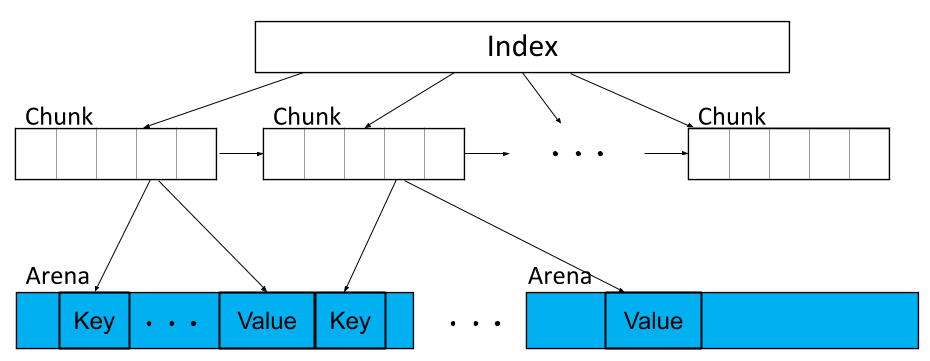
\includegraphics[width=\textwidth]{layout.png}
\caption{Index, chunks, and arenas}
%: the index and chunk list are on heap, whereas keys and values are allocated in off-heap arenas.
\label{fig:index}
\end{subfigure}
\hfill
\begin{subfigure}{0.515\linewidth}
\centering
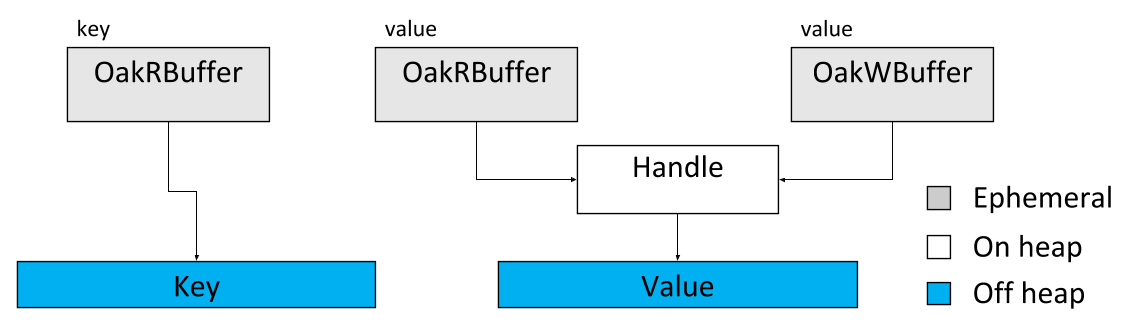
\includegraphics[width=\textwidth]{handle.png}
\caption{Buffers, handles, and data}
\label{fig:handle}
\end{subfigure}
\caption{\oak\ data organization.}
\end{figure*}

% \paragraph{Chunks and index.} 
Oak's on-heap metadata maps keys to values. It
is organized as a linked list of \emph{chunks} -- large blocks of contiguous key ranges, as  in \cite{chunks}. 
Each chunk has a \emph{minKey}, which is invariant throughout its lifespan.
We say that key $k$ is in the \emph{range of chunk $C$} if $k \geq C.$\emph{minKey} and $k < C.next.$\emph{minKey}.

A chunk includes a linked list of \emph{entries},  
%organized as an array-based linked list, 
sorted in ascending key order. 
The entries point to off-heap keys and values. 
%Each entry holds 
%(1) a pointer to a key (off-heap), 
%(2) a pointer to a handle (in the same chunk, on-heap) that points to an off-heap value, 
%and the index of the entry that holds the next key in the linked list. 
\oak\ makes sure that each key appears in at most one entry.


To allow fast access, we follow the approach of \cite{the-art-of,index-1,index-2,kiwi,transactional-lib} and add an \textit{index} 
that maps minKeys to their respective chunks, as illustrated in \Cref{fig:index}. %Each chunk is indexed according to its minKey. 
The index %offers standard lookup, insert, and remove operations. It
is updated in a lazy manner, and so it may be inaccurate, in which case, locating a chunk may involve a partial 
traversal of the chunk linked list. % (as in \cite{kiwi}). 
A \algvar{locateChunk(k)} method returns the chunk whose range includes  key \algvar{k} by querying the index and traversing the chunk list if needed. 

%\paragraph{Intra-chunk organization.}
% As shown in Figure~\ref{fig:chunk}, chunks hold three types of objects: entries, keys, and handles. 



%Given that the prefix and the remainder are of similar sizes, the expected search time remains polylogarithmic. 
%Nevertheless, in the worst-case, the search time is linear in the size of the remainder of the chunk. 

\remove{
\begin{figure}
\centering
\includegraphics[scale=0.4]{chunk.png}
\caption{Oak intra-chunk organization.}
\label{fig:chunk}
\end{figure}
}

\subsection{Memory management}
\label{ssec:mm} 

\oak\ offers a simple default memory manager  that can be overridden by applications.
The default manager  is suitable for real-time analytics settings, where  
dynamic data structures  used to ingest new data  exist for limited time~\cite{Druid,hbase} and
%The operations are mostly inserts and in-situ updates, while 
deletions are infrequent.
%, which motivates the following simple design.  

%Memory management involves two aspects -- {allocation} and GC. 
\oak's allocator manages a shared pool 
of large  (100MB by default) pre-allocated off-heap {\em arenas}, and supports multiple \oak\ instances.  
Each arena is associated with a single \oak\/ instance and returns to the pool when that instance is disposed. 
{Key and value buffers  are allocated from the arena's flat free list 
using a  first-fit approach; they  return to the free list upon KV-pair deletion %(\cref{ssec:handles}) 
or value resize.}

The memory manager can efficiently compute the total size of an \oak\ instance's  off-heap footprint.
%as required by some applications~\cite{HbaseSizeTracking}.


\subsection{Handles and  concurrency control}
\label{ssec:handles}

The handle abstraction provides access to off-heap mutable memory, bridging between the on- and  off-heap parts of \oak,  
as shown in \Cref{fig:handle}. There is a single handle per value, which the  
\algvar{OakRBuffer} and \algvar{OakWBuffer} objects  wrap. Keys are immutable, so their 
\algvar{OakRBuffer}s reference off-heap memory directly, without handles.  
%
Since the handle is an on-heap object, it remains reachable to  threads that hold \oak\ buffers that wrap it 
 after the value  (off-heap) is reclaimed. 



%The handle has the same interface as a Java ByteBuffer, as do the values, which makes them amenable to off-heap allocation. 
The handle ensures that all methods are applied to the buffers atomically. 
The default implementation uses a read-write lock, but can be overridden, e.g., by an optimistic approach.
The handle also interacts with the memory manager in order to dynamically resize values
(requesting a new allocation and copying the buffer to it if needed), 
and informs it when to reclaim buffers that are no longer needed.
%The memory manager is a separate module and is also replaceable.

Once a value is removed from Oak, the handle assures that no thread will attempt to read it, since 
that memory may be reclaimed. 
To this end, the handle performs a logical remove by marking itself as deleted.
A key is deemed present in Oak only if it is associated with a non-deleted handle.
%All other handle operations check if the handle is deleted before taking any action.
% 
The handle further offers 
update and compute mechanisms that are used by \oak\/ to atomically modify values.
%The former directs the handle to  reference to the given value, whereas the latter executes a user-provided lambda, while ensuring that the update occurs 


		
    \section{Oak Algorithm}
    \label{sec:alg}
    
\setlength{\textfloatsep}{0.75\baselineskip}

We now describe the \oak\ algorithm. The ZC  and  legacy  API implementations share the most of it. 
We focus here on the ZC variant; supporting also the legacy API mainly entails serialization and deserialization.

%\oak\ uses chunk objects that support rebalancing; 
We begin in \Cref{ssec:chunks} with an overview  of  chunk objects.  We then proceed to describe  \oak's operations.
In \Cref{ssec:queries} 
we discuss Oak's queries, namely \algvar{get} and scan.
%Oak's support for various conditional and unconditional updates raises some subtle interactions that need to be handled with care. 
We divide our discussion of update operations into two types: insertion operations that may add a new value to Oak are discussed in 
\Cref{ssec:doput}, whereas operations that only take actions  when the affected key is already in Oak are given in 
\Cref{ssec:doIfPresent}.
%given in Algorithm~\ref{alg:doput}, whereas \algvar{remove} and \algvar{computeIfPresent}, which only take actions  when the affected key is in Oak, are given in Algorithm~\ref{alg:doIfPresent}.
To argue that Oak is correct, we identify  in \Cref{sec:lp} \emph{linearization points} for all operations, so that concurrent operations appear to execute in the order of their linearization points. 
A formal correctness proof is given in the supplementary material. 

%The algorithm makes use of commodity atomic hardware operations like CAS and F\&A.

\subsection{Chunk objects}
\label{ssec:chunks}


A chunk object exposes methods for searching, allocating, and writing, as we describe in this section.
In addition, the chunk object has a  \emph{rebalance} method, which splits chunks when they are over-utilized, merges chunks when they are under-used, and reorganizes chunks' internals. 
Our rebalance is implemented as in previous   constructions \cite{kiwi,Braginsky-BTree}.
Since it is not novel and orthogonal to our contributions, we do not detail it, but rather outline its guarantees.
Implementing the remaining chunk methods is straightforward.

When a new chunk is created (by rebalance), some prefix of the entries array is filled with data, and the suffix consists of empty entries for future allocation. 
The full prefix is  sorted, that is, the linked list successor of each entry is the ensuing entry in the array. The sorted prefix can be searched efficiently using binary search. 
When a new entry is inserted, it is stored in the first free cell and connected via a bypass in the sorted linked list. If insertion order is random, inserted entries are most likely to be distributed evenly between the ordered prefix entries, keeping the search time low. %, thus creating fairly short bypasses. 

\paragraph{Rebalance guarantees.}
The rebalancer preserves the integrity of the chunks  list in the following sense: Consider a 
\algvar{locateChunk}($k0$) operation that returns $C_0$ at some time $t_0$ in a run, 
and a traversal of the linked list using {next} pointers from $C_0$ reaching a chunk whose range 
ends with $k1$ at time $t_1$. For each traversed chunk $C$, choose an arbitrary time $t_0 \le t_C \le t_1$ and 
consider the sequence of keys stored in $C$ at time $t_C$. 
Let $T$ be the concatenation of these sequences. 
Then:
\begin{description}
    \item[RB1] $T$ includes every key $k \in [k0,k1]$ that is inserted before time $t_0$ 
		and is not removed before time $t_1$; 
    \item[RB2] $T$ does not include any key that is either not inserted before time $t_1$ or is 
		removed before time $t_0$ and not re-inserted before time $t_1$; and 
    \item[RB3]   $T$ is sorted  in monotonically increasing order.
\end{description}

\paragraph{Chunk methods.}



 %\algvar{lookUp}, \algvar{allocateEntryAndKey, allocateHandle, entriesLLputIfAbsent, writeValue, publish}, and \algvar{unpublish}.
% We now describe their operation; their implementation is straightforward (except for rebalancing) and so we omit it from the pseudo-code. 
The chunk's 
\algvar{LookUp(k)} method searches for an entry corresponding to  key \algvar{k}. 
This is done by first running a binary search on the entries array prefix and continuing the search by traversing the entries linked list. 
Note that \oak\ ensures that there is at most one relevant entry.

We rely on three allocation methods:
\algvar{allocateHandle} allocates a new handle;  
\algvar{allocateEntryAndKey} allocates a new entry and also allocates and writes the given key that it points to (off-heap); and
\algvar{writeValue} allocates space for the value (outside the chunk), writes the value to it, and links the handle to the value.
Allocations use atomic hardware operations like F\&A, so that the same space is not allocated twice.
%
%A new entry can be  added to the entries linked list by 
\algvar{entriesLLputIfAbsent} adds an entry to the linked list; it uses CAS in order 
to preserve the invariant of a key not appearing more than once.
If it encounters an  entry with the same key, then it returns the encountered entry.

In-chunk allocations (of handles and entries) may trigger a rebalance ``under the hood''. 
In this case, the allocate procedure fails returning $\bot$ and Oak retries the update. 
While a chunk is being rebalanced, calls to \algvar{entriesLLputIfAbsent} fail and return $\bot$.

Update operations inform the rebalancer of the action they are about to perform on the chunk by calling the \algvar{publish} method.
This method, too, fails in case the chunk is being rebalanced. 
In principle,  rebalance may help published operations complete (for lock-freedom), but for simplicity, our description 
herein assumes that it does not. Hence, we always retry an operation upon failure.
When the update operation has finished its published action, it calls \algvar{unpublish}. 
%We implement the publish and unpublish methods as in KiWi~\cite{kiwi}. 

Whereas chunk update methods that encounter a rebalance fail (return $\bot$),  methods that do not modify the entries list proceed concurrently with rebalance without aborting.
This includes \algvar{lookUp}, \algvar{writeValue}, and \algvar{unpublish}.  

% 


\subsection{Queries -- get and scans} 
\label{ssec:queries}


%\paragraph{Get.}
The \algvar{get} operation is given in \Cref{alg:get}. 
It returns a read-only view (\algvar{oakRBuffer}) of the handle that holds the value that is mapped to the given key. %, in accordance with our zero-copy policy.
Since it is only a view and not a copy of the value, if the value is then updated by a different operation, the view will refer to the updated value. 
%The returned view cannot be used for updating the value since it is a read-only view.
%Consistency is achieved by making sure that ByteBuffer operations performed on the oakBuffer are thread-safe, for example, we can use a read-write lock in the handle for concurrency control. 
Furthermore, a concurrent operation can remove the key from Oak, in which case the handle will be marked as deleted;  reads from the \algvar{oakRBuffer}  check this  flag
and throw an exception in case the value is deleted. 



\begin{algorithm}[tb]
\small
\caption{Get}
\label{alg:get}
\begin{algorithmic}[1]
\Procedure{get}{\key}
\State \algvar{C}, \algvar{ei}, \algvar{hi}, \algvar{handle} $\assign \bot$
\State \algvar{C} $\assign$ locateChunk(\key)  \label{line:locate chunk}; 
%\State 
\algvar{ei} $\assign$ \algvar{C}.lookUp(\key) \label{line:lookup}
\If {$\algvar{ei} \neq \bot$}  $\algvar{hi} \assign$ \algvar{C.entries[ei].hi}
\EndIf \label{line:get ei}
\If {$\algvar{hi} \neq \bot$} $\algvar{handle} \assign $\algvar{C.handles[hi]}
\EndIf \label{line:get hi}
\If {$\algvar{handle} = \bot \ \lor \ \algvar{handle.deleted} $} \Return \NULL \label{line:get check deleted}
\Else \ \Return new OakRBuffer(\algvar{handle})
\EndIf
\EndProcedure
\algstore{getHandle}
\end{algorithmic}
\end{algorithm}

The algorithm first locates the relevant chunk and calls lookUp (line~\ref{line:lookup}) to search for an entry with the given key.
Then, it finds the handle and checks if it is deleted. % (line~\ref{line:get check deleted}).
If an entry holding a valid and non-deleted handle is found, it creates a new \algvar{oakRBuffer} that points to the handle and returns it. Otherwise, \algvar{get} returns \textsc{null}.

%\paragraph{Scan.}
The ascending scan begins by locating the first chunk with a relevant key in the scanned range using \algvar{locateChunk}. 
It then traverses the entries within each relevant chunk using the intra-chunk entries linked list, and continues to the next chunk in the chunks linked list. 
The iterator returns an entry it encounters only if its handle index is not $\bot$ and the handle is not deleted. Otherwise, it continues to the next entry.

The descending iterator begins by locating the \emph{last} relevant chunk.
Within each relevant chunk, it first locates the last relevant entry in the sorted prefix, and then 
scans the (ascending) linked list from that entry until the last relevant entry in the chunk, while saving the entries it traverses in a stack.
After returning the last entry, it pops and returns the stacked entries.  
Upon exhausting the stack and reaching an entry in the sorted prefix, the iterator simply proceeds to the previous prefix entry (one cell back in the array) and rebuilds the stack with the linked list entries in the next bypass. 


\begin{figure}[tb]
\centering
\includegraphics[scale=0.4]{../figures/descend_entries.png}
\hspace{5mm}
\includegraphics[scale=0.4]{../figures/descend_stacks.png}
\caption{Example entries linked list (left) and stacks built during its traversal by a descending scan (right).}
\label{fig:descend}
\end{figure}

\Cref{fig:descend} shows an example of an entries linked list and the stacks constructed during its traversal.
In this example, the ordered prefix ends with~9, which does not have a next entry, so we  can return it.
Next, we move one entry back in the prefix, to entry~6, and traverse the linked list until returning to an already seen entry within the prefix (9~in this case), 
while creating the stack 8~$\rightarrow{}$~7~$\rightarrow{}$~6. 
We then pop and return each stack entry.
Now, when the stack is empty, we again go one entry back in the prefix and traverse the linked list. Since after~5 we reach~6, which is also in the prefix, we can return~5. 
Finally, we reach~2 and create the stack with entries 4~$\rightarrow{}$~3 $\rightarrow{}$~2, which we pop and return. 
When exhausting a chunk, the descending  scan queries the index again, but now for a the chunk with the greatest minKey that is strictly smaller than the current chunk's minKey.
%From the chunk returned by the index, we again traverse the chunks linked list until the last chunk with a smaller minKey than the last key the iterator returned.


\newenvironment{enum}%
  {\begin{enumerate}%
      \setlength{\partopsep}{0pt}%
      \setlength{\topsep}{0pt}%
    \setlength{\itemsep}{0pt}%
    \setlength{\parsep}{0pt}}%
  {\end{enumerate}}

%\paragraph{Iterator correctness.}
By RB1-3 it is easy to see that the scan algorithm described above guarantees the following:
\begin{enumerate} 
    \item A scan returns all relevant keys that were inserted to Oak before the start of the scan and not removed until its end.
    \item A scan does not return keys that were never present or were removed from Oak before the start of the scan and not inserted until it ends.
    \item A scans does not return the same key more than once.
\end{enumerate}

Note that relevant keys inserted or removed concurrently with a scan may be either included or excluded.

\subsection{Insertion operations} 
\label{ssec:doput}

The three insertion operations --  \algvar{put, putIfAbsent}, and  \algvar{putIfAbsentComputeIfPresent} -- use  the \algvar{doPut} function in \Cref{alg:doput}.
\algvar{DoPut} first locates the relevant chunk and searches for an entry. We then distinguish between two cases: if a non-deleted handle is found (case 1: lines~\ref{line:handle.deleted}~--~\ref{line:doput end case 1}) then we say that the key is \emph{present}.
In this case, \algvar{putIfAbsent} returns \texttt{false} (line~\ref{line:putIf returns false}), \algvar{put} calls handle.put (line~\ref{line:handleput}) to associate the new value with the key, and \algvar{putIfAbsentComputeIfPresent}  calls handle.compute (line \ref{line:handlecompute}). 
The  handle operations return \texttt{false} if the handle is deleted (due to a concurrent remove), in which case we retry (line~\ref{line:doputretry}).



\remove{ 
try to associate the given key with  a new value 
%if it is not already associated with a value.
\algvar{putIfAbsent} returns \texttt{true} in this case.
In case the key is present, \algvar{putIfAbsent} returns \texttt{false}, \algvar{put}  associates the new value with the key, and \algvar{putIfAbsentComputeIfPresent} 
computes a new value to be associated with the key. 
}


\begin{algorithm}[htb]
\setlength\belowcaptionskip{0pt}
\setlength\abovecaptionskip{0pt}
\small
\caption{Oak's insertion operations}
\label{alg:doput}
\begin{algorithmic}
\algrestore{getHandle}
\Procedure{put\textnormal{(\key,\ \givenvalue)}}{}
\State doPut(\key,\ \givenvalue,\ $\bot$,\ \textsc{put})
\State \Return 
\EndProcedure

\Procedure{putIfAbsent}{\key,\ \givenvalue}
\State \Return doPut(\key,\ \givenvalue,\ $\bot$,\ \textsc{putIf})
\EndProcedure


\Procedure{putIfAbsentComputeIfPresent}{\key,\ \givenvalue,\ \algvar{func}}
\State doPut(\key,\ \givenvalue,\ \algvar{func},\ \textsc{compute})
\State \Return 
\EndProcedure
\Statex
\Procedure{doPut}{\key,\ \givenvalue,\ \algvar{func},\ \algvar{operation}}
\State \algvar{C}, \algvar{ei}, \algvar{hi}, \algvar{newHi}, \algvar{handle} $\assign \bot$; \algvar{result}, \algvar{succ} $\assign$ true
\State \algvar{C} $\assign$ locateChunk(\key); 
%\State 
\algvar{ei} $\assign$ \algvar{C}.lookUp(\key)
\If {$\algvar{ei} \neq \bot$}  $\algvar{hi} \assign$ \algvar{C.entries[ei].hi}
\EndIf
\If {$\algvar{hi} \neq \bot$} $\algvar{handle} \assign $\algvar{C.handles[hi]}
\EndIf
\If {$\algvar{handle} \neq \bot \ \land \ \neg\algvar{handle.deleted}$} 
\LeftComment{Case 1: key is present}
 \label{line:handle.deleted}
\If {$\algvar{operation} = \textsc{putIf}$} \Return false \label{line:putIf returns false}
\EndIf
\If {$\algvar{operation} = \textsc{put}$} \algvar{succ} $\assign$ \algvar{handle}.put(\givenvalue) \label{line:handleput}
\EndIf
\If {$\algvar{operation} = \textsc{compute}$} 
\State \algvar{succ} $\assign$ \algvar{handle}.compute(\algvar{func}) \label{line:handlecompute}
\EndIf
\If {$\neg\algvar{succ}$} 
\State \Return doPut(\key,\ \givenvalue,\ \algvar{func},\ \algvar{operation}) \label{line:doputretry}
\EndIf
\State \Return true \label{line:doput end case 1}
\EndIf
\LeftComment{Case 2: key is absent}
\If {$\algvar{ei} = \bot$}
\State \algvar{ei} $\assign$ \algvar{C}.allocateEntryAndKey(\key) \label{line:allocateentry}
\State $\algvar{ei} \assign $\algvar{C}.entriesLLputIfAbsent(\algvar{ei}) \label{line:linkentry}
\EndIf
\State $\algvar{newHi} \assign $\algvar{C}.allocateHandle() \label{line:allocatehandle}
\If {$\algvar{ei} = \bot \lor \algvar{newHi} = \bot$} \label{line:nospace} 
\Comment{allocation or insertion failed}
\State
\Return doPut(\key,\ \givenvalue,\ \algvar{func},\ \algvar{operation})

\EndIf 
\State \algvar{C}.writeValue(\algvar{newHi},\ \givenvalue) \label{line:writevalue}
\If {$\neg$\algvar{C}.publish(\algvar{ei},\ \algvar{hi},\ \algvar{newHi},\ \algvar{func},\ \algvar{operation})} 
\State \Return doPut(\key,\ \givenvalue,\ \algvar{func},\ \algvar{operation})
\EndIf \label{line:publish}
\State \algvar{result} $\assign$ CAS(\algvar{C}.\algvar{entries[ei].hi}, \algvar{hi}, \algvar{newHi}) \label{line:cashandle}
\State \algvar{C}.unpublish(\algvar{ei},\ \algvar{hi},\ \algvar{newHi},\ \algvar{func},\ \algvar{operation}) \label{line:unpublish}
\If {$\neg\algvar{result}$} \label{line:retryaftercas} 
\State \Return doPut(\key,\ \givenvalue,\ \algvar{func},\ \algvar{operation}) \label{line:doputretryatend}
\EndIf
\State \Return true \label{line:doput return}
\EndProcedure
\algstore{doPut}
\end{algorithmic}
\end{algorithm}



In the second case, the key is absent.
If we discover a removed entry that points to the same key but with $\algvar{hi} = \bot$ or a deleted handle, then we reuse this entry. 
Otherwise, we call \algvar{allocateEntryAndKey} to allocate a new entry as well as allocate and write the key that it points to (line~\ref{line:allocateentry}), and 
then  try to link this new entry into the entries linked list  (line \ref{line:linkentry}).
Either way, we allocate a new handle (line~\ref{line:allocatehandle}).
These functions might fail and cause a retry (line~\ref{line:nospace}).

If \algvar{entriesLLputIfAbsent} receives $\bot$ as a parameter (because the allocation in line~\ref{line:allocateentry} fails) then it just returns $\bot$ as well. 
Otherwise, if it encounters an already linked entry then it returns it.
In this case, the entry allocated in line~\ref{line:allocateentry} remains unlinked in the entries array and other operations never reach it; the rebalancer eventually removes it from the array.
After allocations of the entry, key, and handle, we allocate and write the value (outside the chunk), and have the new handle point to it (line \ref{line:writevalue}).

We complete the insertion by using CAS to make the entry point to the new handle index (line~\ref{line:cashandle}). 
Before doing so, we publish the operation (as explained in \cref{ssec:chunks}), 
which can also lead to a retry (line \ref{line:publish}).
After the CAS, we unpublish the operation, as it is no longer pending (line~\ref{line:unpublish}). 
If CAS fails, we retry the operation (line~\ref{line:doputretryatend}). 

To see why we retry, observe that the CAS may fail because of a concurrent non-insertion operation that sets the handle index to $\bot$ or because of a concurrent insertion operation that sets the handle index to a different value.
In the latter case, we cannot order (linearize) the current operation before the concurrent insertion, because the concurrent insertion operation might be a \algvar{putIfAbsent}, and would have returned \texttt{false} had the current operation preceded it.

\begin{algorithm*}[htb]
\small
\setlength\multicolsep{0pt}
\caption{Oak's non-insertion update operations}
\label{alg:doIfPresent}
\begin{algorithmic}[1]
\algrestore{doPut}
\begin{multicols}{2}
\Procedure{doIfPresent}{\key,\ \algvar{func},\ \algvar{op}}
\State \algvar{C}, \algvar{ei}, \algvar{hi}, \algvar{handle} $\assign \bot$; \algvar{res} $\assign$ true
\State \algvar{C} $\assign$ locateChunk(\key);  
%\State 
\algvar{ei} $\assign$ \algvar{C}.lookUp(\key)
\If {$\algvar{ei} \neq \bot$}  $\algvar{hi} \assign$ \algvar{C.entries[ei].hi}
\EndIf
\If {$\algvar{hi} = \bot$} \Return false
\EndIf \label{line:doIfPresent hi is bot}
\State $\algvar{handle} \assign $\algvar{C.handles[hi]}
\If {$\neg\algvar{handle.deleted}$} \LeftComment{Case 1: handle exists and not deleted} \label{line:doIfPresent reads deleted}
\If {\algvar{op} = \textsc{comp}  $\land$ \algvar{handle}.compute(func)}  \label{line:doIfPresent handle compute return true}
\State \Return true
\EndIf
\If {\algvar{op} = \textsc{rm} $\land$  \algvar{handle}.remove()} \label{line:doIfPresent handle remove}
\State \Return finalizeRemove(\algvar{handle})
\EndIf
\EndIf
\LeftComment{Case 2: handle is deleted -- ensure key is removed}
\If {$\neg$\algvar{C}.publish(\algvar{ei},\ \algvar{hi},\ $\bot$,\ \algvar{func},\ \algvar{op})} 
\State \Return doIfPresent(\key,\ \algvar{func},\ \algvar{op})
\EndIf \label{line:doIfPresent publish}
\State \algvar{res} $\assign$ CAS(\algvar{C}.\algvar{entries[ei].hi}, \algvar{hi}, $\bot$) \label{line:doIfPresent cas}
\State \algvar{C}.unpublish(\algvar{ei},\ \algvar{hi},\ $\bot$,\ \algvar{func},\ \algvar{op})
\If {$\neg\algvar{res}$} 
\Return doIfPresent(\key,\ \algvar{func},\ \algvar{op}) \label{line:doIfPresent retry}
\EndIf
\State \Return false \label{line:doIfPresent final return false}
\EndProcedure

%\columnbreak

\Procedure{computeIfPresent}{\key,\ \algvar{func}}
\State \Return doIfPresent(\key,\ \algvar{func},\ \textsc{comp})
\EndProcedure
\Statex
\Procedure{remove}{\key}
\State doIfPresent(\key,\ $\bot$,\ \textsc{rm})
\State \Return 
\EndProcedure
\Statex
\Procedure{finalizeRemove}{\algvar{prev}}
\State \algvar{C}, \algvar{ei}, \algvar{hi}, \algvar{handle} $\assign \bot$
\State \algvar{C} $\assign$ locateChunk(\key);  
%\State 
\algvar{ei} $\assign$ \algvar{C}.lookUp(\key)
\If {$\algvar{ei} \neq \bot$}  $\algvar{hi} \assign$ \algvar{C.entries[ei].hi}
\EndIf
\If {$\algvar{hi} = \bot$} \Return true
\EndIf 
\State $\algvar{handle} \assign $\algvar{C.handles[hi]}
\If {$\algvar{handle} \neq \algvar{prev}$} \Return true 
\label{line:finalizeRemove prev neq handle}
\EndIf
\If {$\neg$\algvar{C}.publish(\algvar{ei}, \algvar{hi}, $\bot$, $\bot$, \textsc{rm})} 
\State \Return finalizeRemove(\algvar{prev})
\EndIf
\State CAS(\algvar{C}.\algvar{entries[ei].hi}, \algvar{hi}, $\bot$) \label{line:finalizeRemove cas}
\State \algvar{C}.unpublish(\algvar{ei},\ \algvar{hi},\ $\bot$,\ $\bot$,\ \textsc{rm})
\State \Return true
\EndProcedure
\end{multicols}
\end{algorithmic}
\end{algorithm*}


\subsection{Non-insertion operations} 
\label{ssec:doIfPresent}

The non-removing updates,  \algvar{computeIfPresent} and \algvar{remove},  
%do not insert new entries. Both 
use the \algvar{doIfPresent} function   in \Cref{alg:doIfPresent}. 
It first locates the handle, and if there is none,  returns \texttt{false} (line~\ref{line:doIfPresent hi is bot}).

In  \algvar{computeIfPresent}, if the handle exists and is not deleted (case 1), we run  handle.compute and return \texttt{true} if it is successful (line~\ref{line:doIfPresent handle compute return true}).
Otherwise (case 2), a subtle race may arise: it is possible for another operation to insert the key after we observe it as deleted and before this point. 
In this case, to ensure correctness, \algvar{computeIfPresent} must assure that the key is in fact removed. 
To this end, it performs a CAS to change handle index to $\bot$ (line~\ref{line:doIfPresent cas}).
Since this affects the chunk's entries, we need to synchronize with a possibly ongoing rebalance,  so we publish before the CAS and unpublish when done. 
If publish or CAS fails then we retry (lines~\ref{line:doIfPresent publish}~and~\ref{line:doIfPresent retry}). 
The operation returns \texttt{false} whenever it does not find the entry, or finds the entry but with $\bot$ as its handle index (line~\ref{line:doIfPresent hi is bot}), or CAS to $\bot$ is successful (line~\ref{line:doIfPresent final return false}).

In \algvar{remove}, 
if a non-deleted handle exists (case 1),  it also updates the handle, in this case, marking it as deleted by calling handle.remove (line~\ref{line:doIfPresent handle remove}), 
and we say that the remove is \emph{successful}.
This makes  other threads aware of the fact that the key has been removed, 
%so there will be no further attempts to read its value, 
which suffices for correctness.
However, as an optimization, \algvar{remove} also performs a second task after marking the handle as deleted, namely, marking the appropriate entry's handle index as $\bot$. 
Updating the entry serves two purposes:
first, rebalance does not check whether a handle is deleted,
so changing the handle index to $\bot$ is needed to allow garbage collection;
second, updating the entry expedites other operations, which do not need to read the handle in order to see that it is deleted. 

Thus, a successful  \algvar{remove}  calls  \algvar{finalizeRemove}, which  tries to CAS the handle index to $\bot$.
We have to take care, however, in case the handle index had already changed, not to change it to $\bot$. 
To this end,  \algvar{finalizeRemove} takes a parameter \algvar{prev} -- the handle  that \algvar{remove} marked as deleted. 
If the entry no longer points to it, we do nothing (line \ref{line:finalizeRemove prev neq handle}).
We save in \algvar{prev} the handle itself and not the handle index, to avoid an ABA problem, since after a rebalance, the handle index might remain the same but reference a different handle. 
Since  \algvar{remove}  is linearized at the point where it marks the handle as deleted, it does not have to succeed in performing the CAS in   \algvar{finalizeRemove}.
If CAS fails, this means that either some insertion operation reused this entry or another non-insertion operation  set the  index to $\bot$.

If  \algvar{remove}  finds an already deleted handle (case 2), it cannot simply return, since by the time remove notices that the handle is deleted, the entry might point to another handle.
Therefore, similarly to \algvar{computeIfPresent}, it makes sure that the key is removed by performing a successful CAS of the handle index to $\bot$ (line~\ref{line:doIfPresent cas}).
In this case (case 2) it does not perform \algvar{finalizeRemove}, but rather retries if the CAS fails (line~\ref{line:doIfPresent retry}).
Note the difference between the two cases: in case 1, we set the handle to deleted, and so changing the entry's handle index to $\bot$ is merely an optimization, and should only occur if the entry still points to the deleted handle. 
In the second case, on the other hand, \algvar{remove} does not delete any handle, and so it \emph{must} make sure that the entry's handle index is indeed $\bot$ before returning. 


\subsection{Linearization points}
\label{sec:lp}

In the supplementary material we show that Oak's operations (except for scans) are \emph{linearizable}~\cite{linearizability}; that is, every operation appears to take place atomically at some point (the linearization point, abbreviated \emph{l.p.}) between its invocation and response.
We now list the linearization points.


\newenvironment{desc}%
  {\begin{description}%
      \setlength{\partopsep}{0pt}%
      \setlength{\topsep}{0pt}%
    \setlength{\itemsep}{0pt}%
    \setlength{\parsep}{0pt}}%
  {\end{description}}

\begin{description}

\item[putIfAbsent] -- if it returns \texttt{true}, the l.p.\ is the successful CAS of handle index (line~\ref{line:cashandle}).
Otherwise, the l.p.\ is when it finds a non-deleted handle
% (reads $\algvar{handle.deleted}=\algvar{false}$) 
(line~\ref{line:handle.deleted}).

\item[put] -- if it inserts a new key, the l.p.\ is the successful CAS of handle index (line~\ref{line:cashandle}).
Otherwise, 
%put replaces the value of a key and
 the l.p.\ is upon %when a non-deleted handle is found and there is 
 a successful nested call to handle.put (line~\ref{line:handleput}).

\item[putIfAbsentComputeIfPresent] -- if it inserts a new key, the l.p.\ is the successful CAS of handle index (line~\ref{line:cashandle}).
Otherwise, 
%it updates the value of a key and 
the l.p.\ is upon 
%when a non-deleted handle is found and there is 
a successful nested call to handle.compute (line~\ref{line:handlecompute}).

\item[computeIfPresent] -- if it returns \texttt{true}, the l.p.\ is 
%when a non-deleted handle is found and there is 
upon a successful nested call to handle.compute (line~\ref{line:doIfPresent handle compute return true}). Otherwise, 
%computeIfPresent returns \texttt{false} and 
the l.p.\ is when the entry is not found, or it is found but with $\bot$ as its handle index (line~\ref{line:doIfPresent hi is bot}), 
or a successful CAS of handle index to $\bot$ (line~\ref{line:doIfPresent cas}).

\item[remove] -- if it is successful, the l.p.\ is when 
%a non-deleted handle is found and 
a successful nested call to handle remove 
%occurs, setting 
sets the handle to deleted (line~\ref{line:doIfPresent handle remove}).
Otherwise, 
%it is not successful and 
the l.p.\ is when the entry is not found, or handle index is $\bot$ (line~\ref{line:doIfPresent hi is bot}), or 
%a deleted handle is found and 
a successful CAS of handle index to $\bot$ occurs (line~\ref{line:doIfPresent cas}).

\item[get] -- if it returns a handle, then the l.p.\ is the read of a non-deleted handle (line~\ref{line:get check deleted}).
If it returns \textsc{null} 
%there are two cases. If 
and there is no relevant entry then the l.p.\ is when \algvar{lookUp} (line~\ref{line:lookup}) returns $\bot$, or when get reads that the handle index is $\bot$ (line~\ref{line:get ei}).
Otherwise, \algvar{get} reads a deleted handle (line~\ref{line:get check deleted}). However, the l.p.\ cannot be the read of the \algvar{deleted} flag in the handle, since by that time, a new handle may have been inserted. 
Instead, 
%Therefore, if  \algvar{get} finds $\algvar{deleted}=\algvar{true}$, then
the l.p.\ is the later between (1) the read of handle index by the same  \algvar{get} (line~\ref{line:get ei}) 
and (2) immediately after the set of  $\algvar{deleted}=\algvar{true}$ by some  \algvar{remove} (note that exactly one \algvar{remove} set deleted to true).

\end{description}


      
    \section{Evaluation}
    \label{sec:eval}

We now evaluate   \oak's Java  implementation using synthetic benchmarks.
In \Cref{sec:druid} below, we discuss a real-world use case.

\subsection{Experiment setup} 

We generate a variety of workloads
using the popular synchrobench  tool~\cite{synchrobench}.
Our hardware testbed features an industry-standard 12-core Xeon E5-4650 CPU with 192 GB RAM. 

\paragraph{Compared solutions.} 
Our ultimate goal is to offer \oak\ as an alternative to Java's standard skiplist. 
We therefore compare it to the JDK8 ConcurrentSkipListMap~\cite{JavaSkipList},
which we refer to as \csl.  
%
To isolate the impact of off-heap allocation from other algorithmic aspects, 
we also implement  an off-heap variant of the Java skiplist, which we call \YoniList.
Note that whereas \csl\ offers an object-based API, \YoniList\ also exposes \oak's ZC API. 
Internally, \YoniList\/ 
maintains a concurrent skiplist over an intermediate {\em cell\/} object. Each cell references a key buffer 
and a value buffer allocated in off-heap arenas  through \oak's memory manager. 
%\YoniList\/ has a bigger on-heap footprint than \oak; however, its ZC API does not have the overhead of creating ephemeral objects upon reads. 
This solution is inspired by off-heap support  in production systems, e.g., HBase~\cite{HbaseOffheapWritePath}. 

{We also experimented with the open source concurrent off-heap B-tree implementation from MapDB~\cite{MapDB}, 
however it failed to scale to big datasets, peforming at least ten-fold slower than \oak; we omit these results for brevity.}

\paragraph{Methodology.}
The exercised keys and values are 100B- and 1KB-big, respectively. 
In each experiment, a specific \emph{range} of keys is accessed. 
Accessed keys are sampled  uniformly at random from that range. 
The range is used to control the dataset size:
Every experiment starts with an {\em ingestion\/} 
stage, which runs in a single thread and populates the KV-map with 50\% of the unique keys in the range 
using \algvar{putIfAbsent} operations. It is followed by the {\em sustained-rate\/} stage, 
which runs the target workload for 30 seconds through one or more symmetric worker threads. 
%
Every data point is the median of 3 runs; {the deviations among runs were all within 10\%}.
%All experiments exploit 32GB RAM, unless stated otherwise. 

In each experiment, all algorithms run with the same RAM budget. 
\oak\/ and \YoniList\/ split the available memory between the off-heap pool and the heap, 
allocating the former with just enough resources to host the raw data. \csl\/ allocates all the 
available memory to heap. 

% \paragraph{Configuration.}
We configure \oak\/ to use 4K entries per chunk, and invoke rebalance whenever the unsorted linked list
exceeds 0.5 of the sorted prefix. The  arena size is 100MB. 

\subsection{Results} 

\begin{figure*}[tb]
\centering
\begin{subfigure}[b]{0.33\linewidth}
\includegraphics[width=\textwidth]{figs/Ingestion.pdf}
\caption{Fixed RAM (32GB), varying dataset}
\label{fig:ingest:fixed_ram}
\end{subfigure}
\hspace{0.1\linewidth}
\begin{subfigure}[b]{0.33\linewidth}
\includegraphics[width=\textwidth]{figs/rev_Ingestion.pdf}
\caption{Fixed dataset (11GB), varying RAM}
\label{fig:ingest:fixed_data}
\end{subfigure}
\caption{Ingestion throughput scaling with RAM, single-threaded execution.}
\label{fig:memscale:ingestion}
\end{figure*}

\paragraph{Memory efficiency.}
We first study  how much of the available RAM can be utilized for the raw data, 
and how fast algorithms can perform within a given memory budget. 
Figure~\ref{fig:ingest:fixed_ram} depicts the  throughput of the ingestion stage 
with 32GB of RAM as the  number of ingested unique 
keys  goes up from 1M (approximately 1.1GB of raw data) to 20M (22GB). 
In Figure~\ref{fig:ingest:fixed_data}, we fix the dataset size to 10M KV-pairs (11GB), and vary the  
RAM budget from 15GB to 26GB.

First, we observe that the off-heap solutions can accommodate  bigger datasets within the same RAM,
and conversely, require less RAM to accommodate the same amount of data. 
For example, with 32GB of RAM,  \csl\/ caps at 15M KV-pairs while the off-heap solutions can accommodate 20M pairs.
This is due to the memory overhead for storing Java objects.
Note  that all algorithms deteriorate as the number of keys rises.
This happens because (1) the search time becomes  slower as the data structure grows, 
and (2) the Java GC overhead increases. 

Second, while the performance of on- and off-heap skiplists is  similar,  \oak\ is significantly faster, especially for large datasets.
There are multiple factors at play here. While off-heap solutions pay an overhead for 
copying all ingested data to off-heap buffers, they also eliminate much of the GC overhead. 
These effects cancel each other out. The  advantage of \oak\ then stems from its 
 locality-friendly data organization. % and low synchronization overhead.  


\paragraph{Scalability with parallelism.}
In the next set of experiments, we fix the available memory to 32GB and the ingested dataset size to 10M KV-pairs. 
We measure the sustained-rate stage throughput for multiple workloads, while scaling the number of worker threads from 1 to 12. 
In this setting, the raw data is less than 35\% of the available memory, i.e., %all algorithms enjoy a large on-heap headroom, hence 
the GC effect in all algorithms is minor. 

%We start from uniform workloads, each performing operations of a single type. 
Figure~\ref{fig:100_put} depicts the results of a put-only workload.
%(i.e., all operations are puts). 
\oak\/ scales 7.7x with 12 threads, while maintaining a 1.5x--1.9x throughput gap over \csl.  
\YoniList\/ is faster than \csl\/ but slower than \oak. 


Figure~\ref{fig:100_putifabsentcomputeifpresent} evaluates \oak's incremental update API, 
where each in-place update modifies 8 bytes of the value. 
In \csl, we invoke the (non-atomic) merge API.
\remove{
Since the Java API does not include \algvar{putIfAbsentComputeIfPresent}, we simulate it by calling first  \algvar{putIfAbsent},
and if it fails, locking the returned object and performing the computation. 
Since the lock is acquired only after 
\algvar{putIfAbsent} fails, the simulated operation is not atomic as in \oak.
}
In this experiment, 
\oak\/ scales 8x with 12 threads, and has 1.4x--1.6x higher throughput than \csl. 

Figure~\ref{fig:100_get} illustrates the get-only workload. Note that after calling get, an application can 
choose how much of the 1KB value to deserialize.  
To provide an upper bound on the impact of copying retrieved data, we also exercise the legacy API for \oak, which
copies the entire value.  We see that copying slows down \oak's performance by 30\%,
although, perhaps surprisingly, it is still faster than \csl. 
When refraining from copying, \oak\/ scales 10x with 12 threads, and consistently outperforms \csl\/ by 1.5x--1.6x.  
%The application-level gain may vary, depending on how much data the application deserializes 
%from the off-heap buffers. The legacy API, which copies all the data, provides the worst-case 
%performance. In this setting, the measured slowdown is approximately 30\% versus the ZC API, 
%which (surprisingly) is still faster than \csl. 
A mix of 95\% gets and 5\% puts (Figure~\ref{fig:put_get}) 
shows similar results: \oak\/ outperforms the competition by up to 1.75x.

\begin{figure*}[tb]
\centering
\begin{subfigure}[b]{0.33\linewidth}
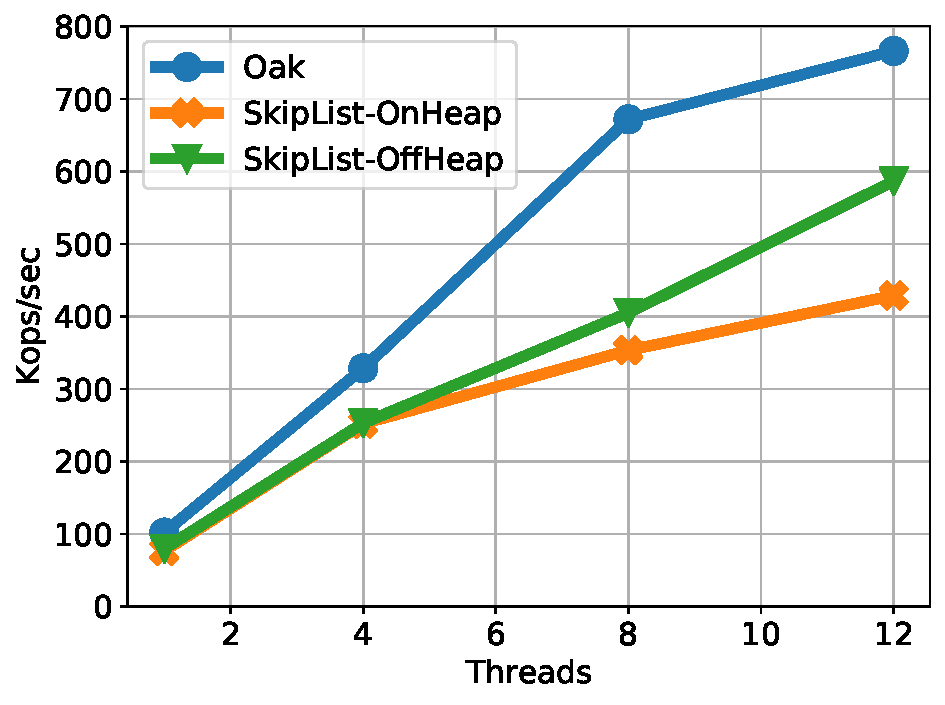
\includegraphics[width=\textwidth]{figs/micro_put-only.pdf}
\vskip -.1in
\caption{Put}
\label{fig:100_put}
\end{subfigure}
\begin{subfigure}[b]{0.33\linewidth}
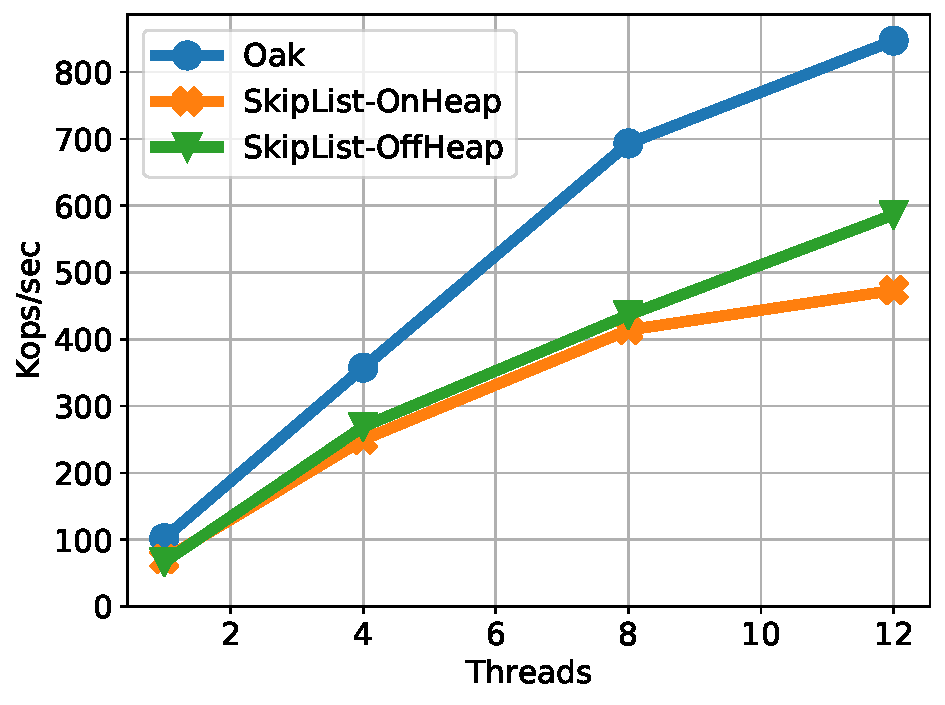
\includegraphics[width=\textwidth]{figs/micro_put-only-computeifpresent.pdf}
\vskip -.1in
\caption{PutIfAbsentComputeIfPresent}
\label{fig:100_putifabsentcomputeifpresent}
\end{subfigure}
\begin{subfigure}[b]{0.33\linewidth}
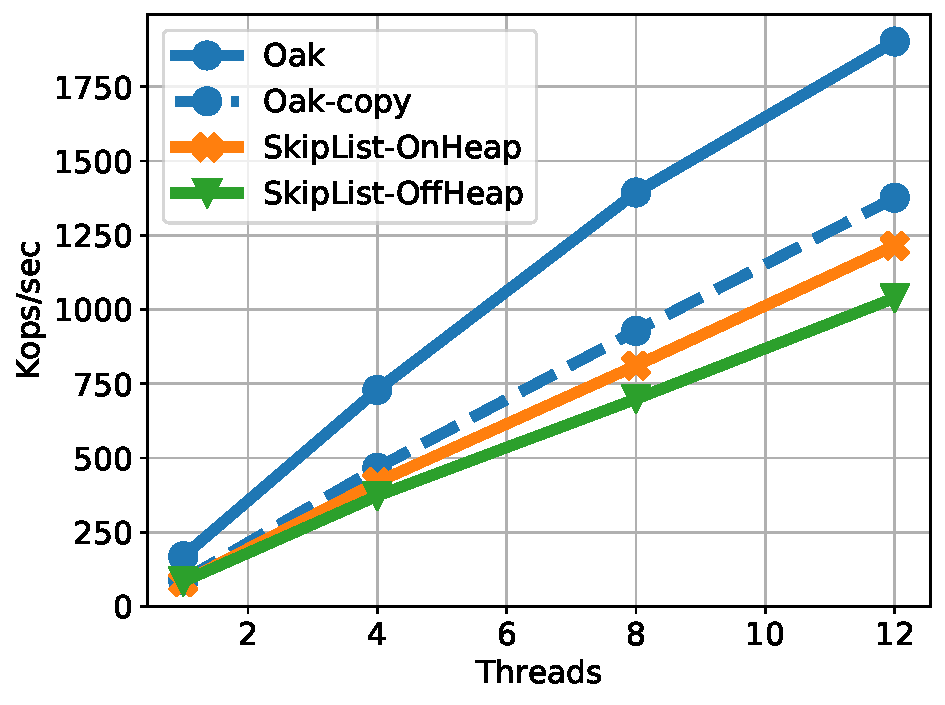
\includegraphics[width=\textwidth]{figs/micro_combined_get-only.pdf}
\vskip -.1in
\caption{Get}
\label{fig:100_get}
\end{subfigure}

\begin{subfigure}[b]{0.33\linewidth}
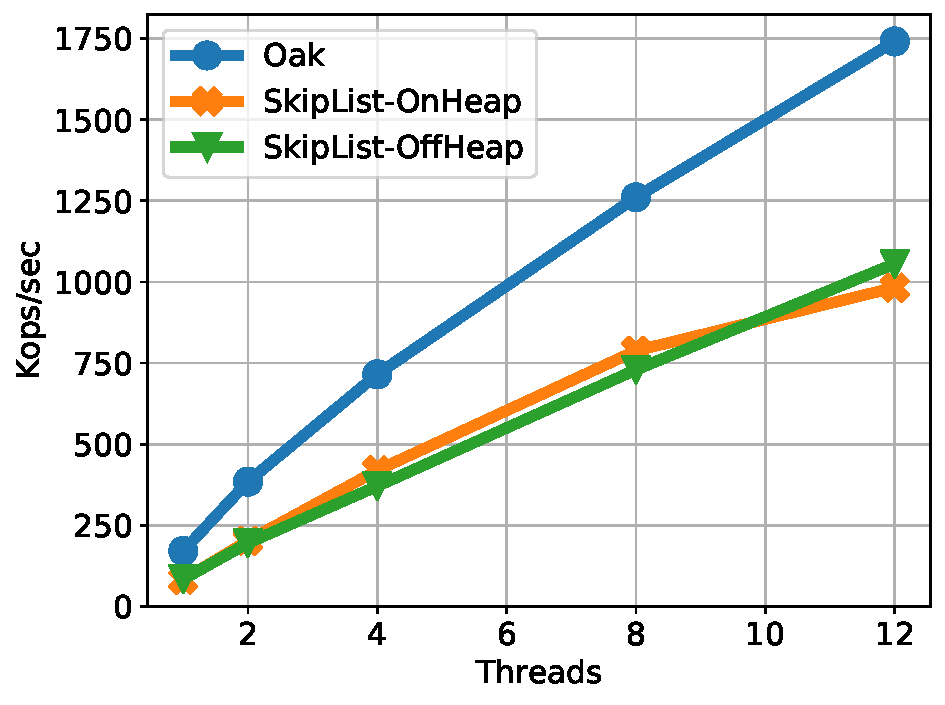
\includegraphics[width=\textwidth]{figs/put_get.pdf}
\vskip -.1in
\caption{95\% get, 5\% put} 
\label{fig:put_get}
\end{subfigure}
\begin{subfigure}[b]{0.33\linewidth}
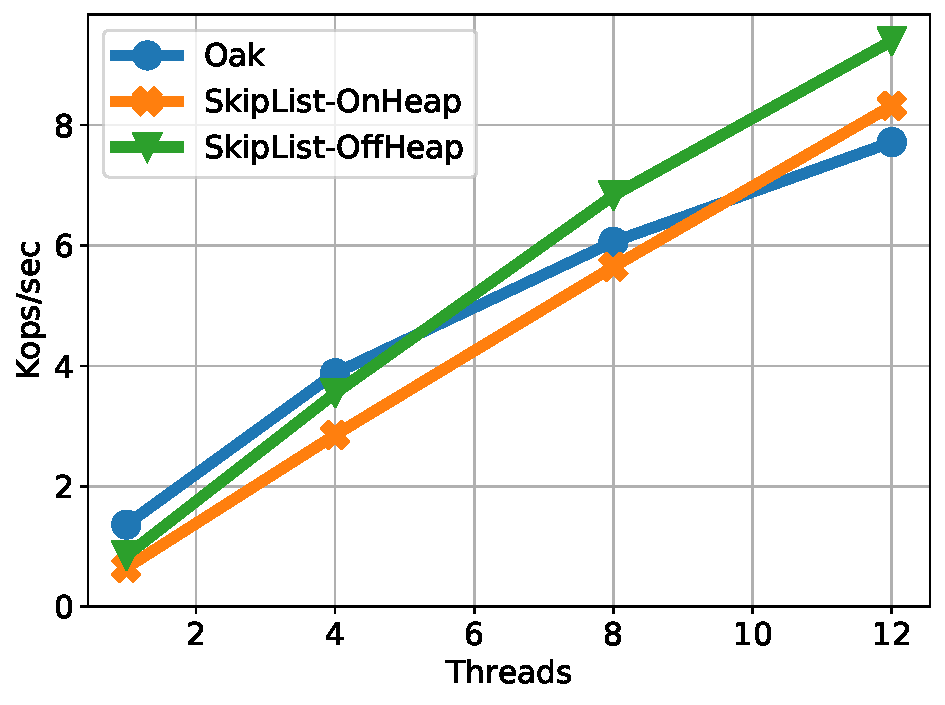
\includegraphics[width=\textwidth]{figs/micro_zc-ascend-only-10k.pdf}
\vskip -.1in
\caption{Scan (ascending), 10K values}
\label{fig:100_ascend_100}
\end{subfigure}
\begin{subfigure}[b]{0.33\linewidth}
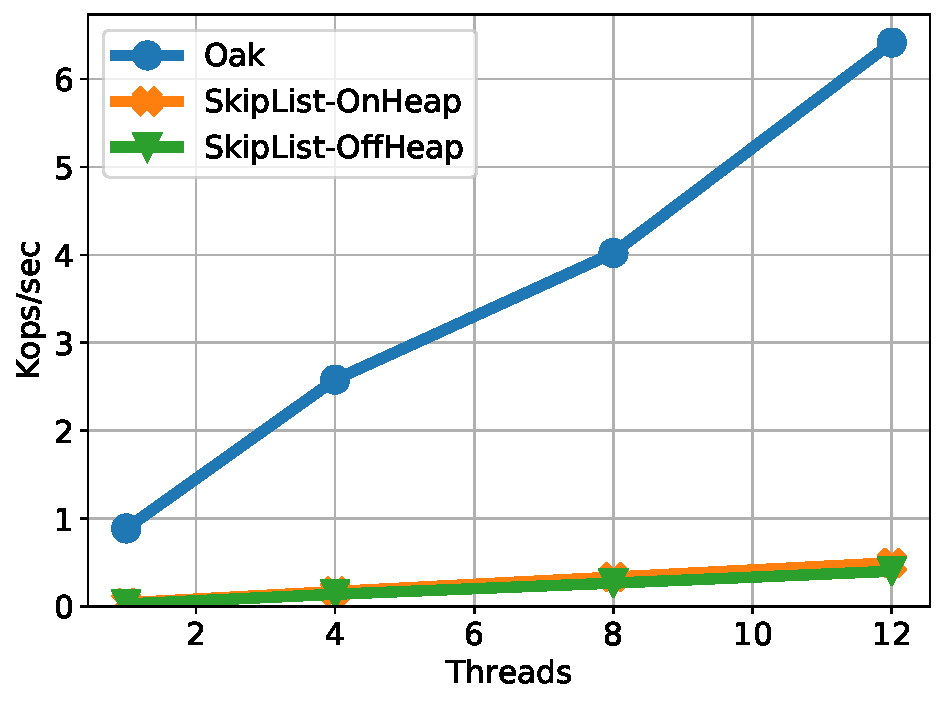
\includegraphics[width=\textwidth]{figs/micro_zc-descend-only-10k.pdf}
\vskip -.1in
\caption{Scan (descending), 10K values}
\label{fig:100_descend}
\end{subfigure}
\label{fig:throughput}
\caption{Sustained-rate throughput scaling with the the number of threads for uniform workloads, 11GB raw data.} 
\end{figure*}

We proceed to  ascending scans. 
%Figure~\ref{fig:100_ascend_10} focuses on short scans that traverse 10 key-value pairs.
Short scans, like gets, are dominated by the search time for the first KV-pair, and so we do not depict them separately. 
% -- e.g., \oak\/ traverses 10 values 40\% faster than \csl.  
Long scans, on the other hand, are dominated by the  iteration through the retrieved pairs.
In such scans, all three solutions perform similarly, as depicted in 
Figure~\ref{fig:100_ascend_100} for scans  traversing 10K values. 


\remove{
In this setting, \oak's performance is aggravated by creation of ephemeral OakRBuffer objects for 
each traversed entity (key, value, or both, depending on the API), whereas its competitors 
only retrieve references to existing objects. Figure~\ref{fig:100_ascend_100} depicts the behavior 
of scans that retrieve either 100 values (solid curve) of 100 KV-pairs (dashed curve). For the former, 
\oak\/ is approximately 20\% faster than \csl\/ (and also \YoniList), whereas for the latter it is 20\% slower, 
as it creates twice as many objects. If the application performs some computation in addition to the raw 
scan, these gaps become immaterial.}

%the overhead of ephemeral object creation and the associated GC are noticeable
%The above results are for raw scan throughput, which does not take any steps during the iteration. 
%We next investigate a scenario where the application executes some computation steps 
%after each key-value pair it retrieves. We use a scan to summarize 100 values, accessing 8 bytes in each of them. 
%As Figure~\ref{fig:100_ascend_compute_100} shows, {\inred {TBC -- wait for Yoni's results.}}
%We studied even longer scans (up to 10K entries), and observed similar throughput losses. %of up to 30\%. 
%Note that Oak has not been designed for this high-intensity read-only setting. %application developers could use a different data structure in this case. 

Finally, Figure~\ref{fig:100_descend} depicts the performance of descending scans over 10K values. 
We see that \oak's efficient chunk-based descending scans are almost as fast as its ascending scans. 
\oak\ exhibits a huge advantage over the competition, outperforming both skiplists more than tenfold. 





 

   \section{Case Study: Druid}
   \label{sec:druid}
\begin{figure*}[tb]
\centering
\begin{subfigure}[b]{0.33\linewidth}
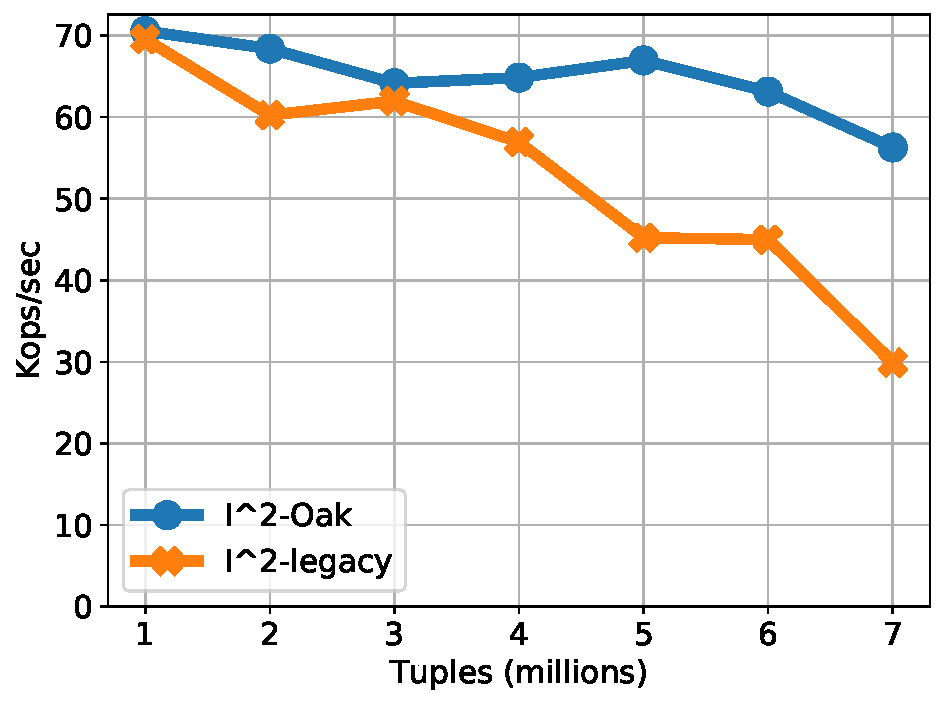
\includegraphics[width=\textwidth]{figs/druid_ingest_30g.pdf}
\vskip -.1in
\caption{Throughput, 30GB RAM, varying dataset}
\label{fig:druid_ingest_32gb_ram}
\end{subfigure}
\begin{subfigure}[b]{0.33\linewidth}
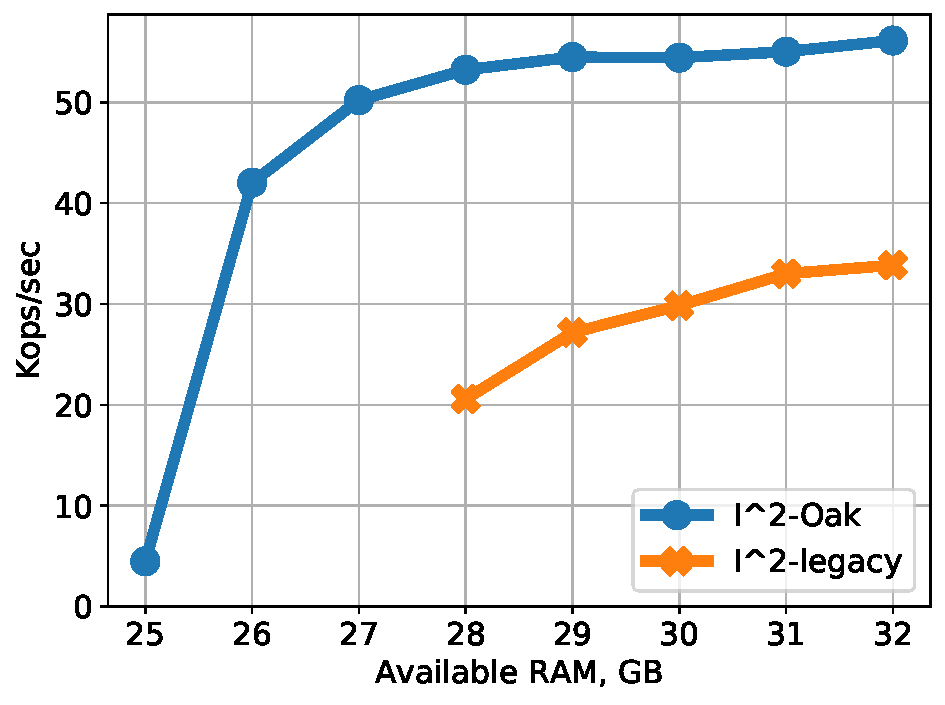
\includegraphics[width=\textwidth]{figs/druid_ingest.pdf}
\vskip -.1in
\caption{Throughput, 7M tuples, varying RAM}
\label{fig:druid_ingest_7m_kv}
\end{subfigure}
\begin{subfigure}[b]{0.33\linewidth}
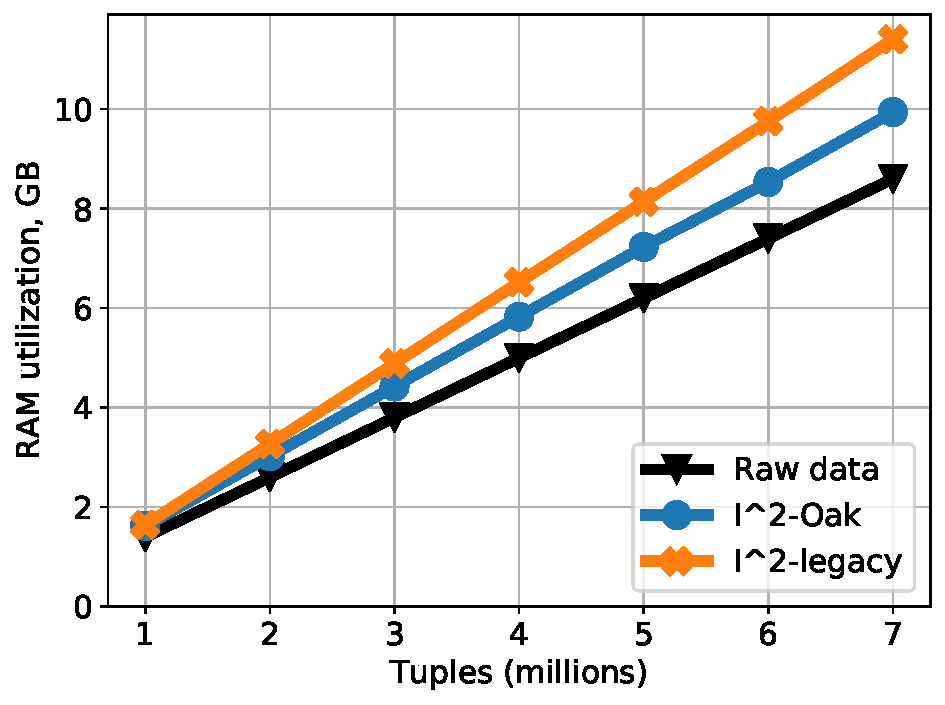
\includegraphics[width=\textwidth]{figs/druid_mem_usage_total.pdf}
\vskip -.1in
\caption{RAM overhead}
\label{fig:druid_mem_usage_total}
\end{subfigure}
\label{fig:druid}
\caption{Single-thread ingestion performance, Druid incremental index: (a,b) throughput, (c) memory efficiency. } 
\end{figure*}

This section presents a case study of \oak's applicability for real-time analytics platforms. 
We build a prototype integration of \oak\ into Apache Druid~\cite{Druid} -- a popular open-source distributed 
analytics database in Java. Our goal is to enable faster ingestion and  improve RAM utilization, which, in turn,  
can lead to I/O reduction. The code, which might be further productized, is under community review~\cite{OakDruidIssue}.

More specifically, we target Druid's \emph{Incremental Index} (\II) component, a  data structure that absorbs new data 
while serving queries in parallel. Data is never removed from an \II. Once an \II\  fills up,  its data gets reorganized and 
persisted, and the \II\ is disposed; the data's further lifecycle is beyond the scope of this discussion. 

\II\/ keys and values are multi-dimensional. In {\em plain\/} \II's, the values are raw data, whereas in {\em rollup\/}
\II's they are materialized aggregate functions. Complex aggregates (e.g., unique count and quantiles) are embodied 
through {\em sketches}~\cite{DruidSketches} -- compact data structures for approximate statistical queries; the rest
are numeric counters. In order to save space, variable-size (e.g., string) dimensions are mapped to numeric codewords, 
through auxiliary dynamic dictionaries. A key maps to a flat array of integers; time is always 
the primary dimension. Keys are typically up to a few hundreds of bytes long. Values are usually up to a few KBs long in 
rollups, and may vary widely in plain indexes. For every incoming data tuple, \II\/ updates its internal KV-map, creating 
a new pair if the tuple's key is absent, or updating in-situ otherwise.

%\paragraph{\oak\/ integration.}  
We re-implement  \II\ by switching the internal map from the JDK ConcurrentSkiplistMap 
to \oak; the auxiliary data structures remain on-heap. 
We implement an adaption layer that controls the internal data layout 
and provides \oak\/ with the appropriate lamdba functions for serialization, deserialization, and in-situ 
compute. The write path exploits \oak's \algvar{putIfAbsentComputeIfPresent()} API for atomic 
update of multiple aggregates within a single lambda. The read path adapts the \II\/ tuple abstraction
to \oak's ZC API. Namely, the new tuple implementation is a lightweight facade to off-heap memory, 
operating atop \oak\/ buffers.

\paragraph{Evaluation.} 
We evaluate the speed and memory utilization of data ingestion with the new solution, \II-\oak,
versus the legacy implementation, \II-legacy. 
The first experiment generates 1M to 7M unique tuples of size 1.25K and feeds them into the index, 
in a single thread. The primary dimension is the current timestamp (in ms), (i.e., the  workload is spatially-local). 
In order to measure ingestion performance in isolation, all the input is generated in advance. 

Figure~\ref{fig:druid_ingest_32gb_ram} depicts the throughput scaling with dataset size, for a fixed RAM budget 
of 30GB. \II-\oak\/ is up to 1.8x faster, e.g., its ingestion speed for 7M tuples (8.6GB 
raw data) is 56K tuples/sec, whereas  \II-legacy's is  30K. Figure~\ref{fig:druid_ingest_7m_kv} 
studies the 7M-tuple dataset under varying memory budget. We see that \II-legacy with 32GB RAM is  more than 25\% slower than
\II-\oak\/ with 26GB RAM, and cannot run with less than 28GB.

Finally, Figure~\ref{fig:druid_mem_usage_total} underscores, \II-\oak's 
memory efficiency. We see that \II-\oak\/ induces at most 15.5\% metadata overhead (including \oak's index and the on-heap 
auxiliary data structures), whereas \II-legacy's space overhead is as high as 32.5\%. 


%Note that \II-\oak's real footprint is much smaller (less than 20GB) because it does not need the 
%pre-generated tuples once they are consumed; \II-legacy references that data from within the index.}





    \section{Conclusion}
    
We presented \oak\/ -- a concurrent ordered KV-map for memory-managed programming platforms like Java. 
%\oak\ is optimized for the real-time big data systems. 
\oak\/ features off-heap memory allocation and GC, in-situ atomic data processing, zero copy API, and internal organization for high speed data access. 
It implements an intricate efficient concurrent algorithm. %, formally proven  correct in the supplementary material.
Multiple benchmarks demonstrate \oak's advantages in scalability and resource efficiency versus the state-of-the-art. 
\oak's code is production quality and open sourced. Its prototype integration with Apache Druid (incubating) demonstrates decisive 
performance gains. 
    
    \newpage
    \bibliography{references}
  
  \appendix
    
    \cleardoublepage
   \section{ Supplementary Material -- Correctness}
    \label{sec:correctness}
In this section, we prove Oak's correctness.
Since the rebalancer is orthogonal to our contribution, we omit it from the discussion of Oak's correctness.
We only assume that RB1-3 hold.
We note that a similar rebalance was fully proven in~\cite{Braginsky-BTree}.

\subsection{Preliminaries}

We consider a shared memory system consisting of a collection of shared variables accessed by threads, which also have local variables.
An \emph{algorithm} defines the behaviors of threads as deterministic state machines, where state transitions are associated with either an instance of a shared variable primitive (read, write, CAS, etc.) or a local step affecting the thread's local variables.
A \emph{configuration} describes the current state of all local and shared variables. An \emph{initial configuration} is one where all variables  hold an initial value.
A data structure implementation provides a set of operations, each with possible parameters. 
We say that operations are \emph{invoked} and \emph{return} or \emph{respond}.
The invocation of an operation leads to the execution of an algorithm by a thread.
Both the invocation and the return are local steps of a thread.
A \emph{run} of algorithm $\mathcal{A}$ is an alternating sequence of configurations and steps, beginning with some initial configuration, such that configuration transitions occur according to $\mathcal{A}$.
We say that two operations are \emph{concurrent} in a run \emph{r} if both are invoked in \emph{r} before either returns.
We use the notion of time \emph{t} during a run \emph{r} to refer to the configuration reached after the $t^{th}$ step in \emph{r}.
An \emph{interval} of a run $r$ is a sub-sequence that starts
with a step and ends with a configuration.
The \emph{interval of an operation} $op$ starts with the invocation step of $op$ and ends with the configuration following the return from $op$ or the end of $r$, if there is no such return.

An implementation of concurrent data structure is \emph{linearizable}~\cite{linearizability} (a correctness
condition for concurrent objects) if it provides the illusion that each invoked operation takes effect instantaneously at some point, called the \emph{linearization point} (l.p.), inside its interval. 
A \emph{linearization} of a run $r$ ($lin(r)$) is the sequential run constructed by serially executing each operation at its l.p.

\subsection{Linearizability proof}

\begin{definition}
\label{def:associated}
If there is an entry $e$ in Oak that points to key $k$ and handle $h$, (i.e., lookUp($k$) returns $e$ s.t. \newline $h=$ \texttt{handles[entries[e].hi]}) and $h\texttt{.deleted = false}$, we say that $h$ is \emph{associated with} $k$.
\end{definition}

\begin{claim}
\label{claim:deleted}
If an Oak operation searches for key $k$ and finds a non-deleted handle $h$ ($\algvar{h.deleted}=\algvar{false}$), then $h$ is associated with $k$.
\end{claim}

\begin{proof}
If an operation searches for $k$ and finds $h$, then there is an entry $e$ that points to $k$, since Oak ensures that there is at most one entry that points to $k$, and $k$ is found only if there is such entry.
This also means that $e$ points to handle $h$ (by handle index $hi$). 
Assume that $e$ does not point to handle $h$, then the handle index is now $hi' \neq hi$.
If $hi'=\bot$ then the handle index can be set only by a non-insertion operation using a CAS. According to Algorithm~\ref{alg:doIfPresent} this is only possible when $h$ in \algvar{handles[$hi$]} is already deleted, but $h$ is not deleted.
Otherwise, $hi' \neq hi$ and $hi' \neq \bot$, then the handle index can be set only by an insertion operation using a CAS. According to Algorithm~\ref{alg:doput} this is only possible when $h$ in \algvar{handles[$hi$]} is already deleted, which is not the case.
Therefore, there is an entry $e$ that points to $k$ and $h$ and $\algvar{h.deleted}=\algvar{false}$, so by Definition~\ref{def:associated} $h$ is associated with $k$.
\end{proof}

\begin{claim}
\label{claim:remove}
Assume handle $h$ is associated with key $k$ at time $t$ in a run $r$.
Then, $h$ is associated with $k$ at time $(t+1)$ in $r$ if and only if the $(t+1)^{st}$ step in $r$ is not the l.p.\ of a successful remove($k$) operation.
\end{claim}

\begin{proof}
Assume that $h$ is not associated with $k$ at time $(t+1)$.  

If there is no handle associated with $k$ at time $t+1$, then by Definition~\ref{def:associated} either $h\texttt{.deleted = true}$ or the entry's handle index ($hi$) is $\bot$.
In the first case, the only possible step that marks a handle as deleted is the l.p.\ of a successful remove($k$).
In the second case, only non-insertion operations turn $hi$ to $\bot$ by using CAS (lines~\ref{line:doIfPresent cas} and \ref{line:finalizeRemove cas}), and according to Algorithm~\ref{alg:doIfPresent} this is only possible when the handle is deleted. 
However, at time $t$, $h$ is still associated with $k$.
Therefore, the entry's handle index ($hi$) is not $\bot$.

Otherwise, there is a different handle $h' \neq h$ that is associated with $k$ at time $t+1$ ($h' \neq
 \bot$).
This change can only be done by an insertion operation using CAS (line~\ref{line:cashandle}). 
According to Algorithm~\ref{alg:doput} an insertion operation reaches that CAS only if the handle ($h$) is already deleted (line~\ref{line:handle.deleted}). 
However, at time $t$, $h$ is still associated with $k$, and so there is no different handle that is associated with $k$.

Therefore, as long as the $(t+1)^{st}$ step is not the l.p.\ of a successful remove($k$), then $h$ is still associated with $k$ at time $t+1$ in $r$, and there is no handle associated with $k$ at time $t+1$ if the $(t+1)^{st}$ step is a l.p.\ of a successful remove($k$), as required.
\end{proof}

\begin{claim}
\label{claim:insert}
Assume no handle is associated with key $k$ at time $t$ in a run $r$.
Then, no handle is associated with $k$ at time $t+1$ in $r$ if and only if the $(t+1)^{st}$ step in $r$ is not the l.p.\ of a successful insertion operation of $k$.
\end{claim}


\begin{proof}
If no handle is associated at time $t$, and at time $t+1$ there is an associated handle, then according to Definition~\ref{def:associated} either a handle's deleted flag turned from false to true, or the entry's handle index turned from $\bot$ to a valid one.
The former is not possible because the handles are initialized as not deleted and only become deleted by a remove; no operation turns a deleted handle to a non-deleted one. 
In the second case, this can only be done by a successful insertion operation, at its l.p.\ (line~\ref{line:cashandle}), as required.
\end{proof}
 

Look at the linearization $lin(r)$ of run $r$ using l.p.s defined in Section~\ref{sec:lp}.
From Claims~\ref{claim:remove} and \ref{claim:insert}, by induction on the steps of a run, we get:
 
\begin{corollary}
\label{corollary}
At any point in a concurrent run $r$, the set of keys associated with handles is exactly the same as the set of inserted keys and not removed keys, associated with the same handles, in $lin(r)$ up to that point.
\end{corollary}


\begin{claim}[Get]
In run $r$, if get($k$) returns $h$ then the corresponding get($k$) in $lin(r)$ returns $h$, and if get($k$) returns \texttt{null} then the corresponding get($k$) in $lin(r)$ returns \texttt{null}.
\end{claim}

\begin{proof}
There are three cases for get's l.p.:
\begin{enumerate}
\item Get($k$) finds a non-deleted handle $h$ (line~\ref{line:get check deleted}), then get($k$) returns $h$ and by Claim~\ref{claim:deleted} $h$ is associated with $k$. 
By Corollary~\ref{corollary}, in $lin(r)$ $k$ is inserted and not removed (the map holds $k$) and since this is the l.p.\ of get then the corresponding get($k$) in $lin(r)$ returns $h$ as well.
\item LookUp($k$) by get($k$) (line~\ref{line:lookup}) returns $\bot$ or if get($k$) reads that the handle index is $\bot$ (line~\ref{line:get ei}), then there is no handle associated with key $k$, and get($k$) returns \texttt{null}.
By Corollary~\ref{corollary}, in $lin(r)$ the map does not hold $k$, and since this is the l.p.\ of get then the corresponding get($k$) in $lin(r)$ returns \texttt{null} as well.
\item Get($k$) finds a deleted handle $h$ at time $t_2$ (line~\ref{line:get check deleted}) and returns \texttt{null}.
Then its l.p.\ is the later between the read of handle index $hi$ by get($k$) at time $t_1 < t_2$ (line~\ref{line:get ei}) and immediately after the set of  $\algvar{deleted}=\algvar{true}$ by remove($k$) at some time $t < t_2$.
Again there are two cases:
\begin{enumerate}
\item If $t > t_1$ then the l.p.\ is immediately after the set of  $\algvar{deleted}=\algvar{true}$ then there is no handle associated with key $k$, and by  Corollary~\ref{corollary}, in $lin(r)$ the map does not hold $k$, and the corresponding get($k$) in $lin(r)$ returns \texttt{null} as well.
\item If $t_1 > t$ then the l.p.\ is the read of handle index $hi$ by get($k$) (line~\ref{line:get ei}) at time $t_1$, after the set of $\algvar{deleted}=\algvar{true}$ at time $t$.
We need to show that at no time between $t$ and $t_1$ the handle index changed to $hi' \neq hi$ and now it does not point to a deleted handle.
Notice that only an insertion operation l.p.\ can change $hi$ to $hi'$.
Assume by contradiction that the l.p.\ of such an operation occurs between $t$ and $t_1$.
Then when get sees $hi$ at time $t_1$, it is already $hi'$ and not $hi$. A contradiction.
Hence, at the l.p.\ of get($k$), there is no handle associated with key $k$, and by Corollary~\ref{corollary}, in $lin(r)$ the map does not hold $k$, so the corresponding get($k$) in $lin(r)$ returns \texttt{null} as required.
\end{enumerate}
\end{enumerate}
\end{proof}


\begin{claim}[PutIfAbsent]
In run $r$, if putIfAbsent($k$) returns \texttt{true} then the corresponding putIfAbsent($k$) in $lin(r)$ returns \texttt{true}, and if putIfAbsent($k$) returns \texttt{false} then in $lin(r)$ the corresponding putIfAbsent($k$) returns \texttt{false}.
\end{claim}

\begin{proof}
If putIfAbsent($k$) finds a non-deleted handle $h$ (line~\ref{line:handle.deleted}), then putIfAbsent($k$) returns \texttt{false} and by Claim~\ref{claim:deleted} $h$ is associated with $k$. 
By Corollary~\ref{corollary}, in $lin(r)$ $k$ is inserted and not removed (the map holds $k$) and since this is the l.p.\ of putIfAbsent then the corresponding putIfAbsent($k$) in $lin(r)$ returns \texttt{false} as well.

Otherwise, if putIfAbsent($k$) performs a successful CAS of handle index from $\bot$ (line~\ref{line:cashandle}), then putIfAbsent($k$) returns \texttt{true} and by Definition~\ref{def:associated} there was no handle associated with $k$ just before the CAS. 
By Corollary~\ref{corollary}, in $lin(r)$ the map does not hold $k$, and since this is the l.p.\ of putIfAbsent then the corresponding putIfAbsent($k$) in $lin(r)$ returns \texttt{true} as required.
\end{proof}

\begin{claim}[ComputeIfPresent]
In run $r$, if computeIfPresent($k$) returns \texttt{true} then in $lin(r)$ the corresponding \newline computeIfPresent($k$) returns \texttt{true}, and if computeIfPresent($k$) returns \texttt{false} then the corresponding computeIfPresent($k$) in $lin(r)$ returns \texttt{false}.
\end{claim}

\begin{proof}
If computeIfPresent($k$) finds a non-deleted handle $h$ and there is a successful nested call to handle compute (line~\ref{line:doIfPresent handle compute return true}), then computeIfPresent($k$) returns \texttt{true} and by Claim~\ref{claim:deleted} $h$ is associated with $k$. 
By Corollary~\ref{corollary}, in $lin(r)$ $k$ is inserted and not removed (the map holds $k$) and since this is the l.p.\ of computeIfPresent then the corresponding computeIfPresent($k$) in $lin(r)$ returns \texttt{true} as well.

If lookUp($k$) by computeIfPresent($k$) returns $\bot$, or if \newline computeIfPresent($k$) reads that the handle index is $\bot$ (line~\ref{line:doIfPresent hi is bot}), then there is no handle associated with key $k$, and \newline computeIfPresent($k$) returns \texttt{false}.
By Corollary~\ref{corollary}, in $lin(r)$ the map does not hold $k$, and since this is the l.p.\ of computeIfPresent then the corresponding computeIfPresent($k$) in $lin(r)$ returns \texttt{false} as required.

Otherwise, a successful CAS of handle index to $\bot$ is performed by computeIfPresent($k$) (line~\ref{line:doIfPresent cas}), from a handle index pointing to a deleted handle (line~\ref{line:doIfPresent reads deleted}).
Then computeIfPresent($k$) returns \texttt{false} and by Definition~\ref{def:associated} there is no handle associated with $k$ just before the CAS and right after it. 
By Corollary~\ref{corollary}, in $lin(r)$ the map does not hold $k$, and since this is the l.p.\ of computeIfPresent then the corresponding computeIfPresent($k$) in $lin(r)$ returns \texttt{false}.
\end{proof}

\begin{claim}[Put]
In run $r$, if put($k$) inserts $k$ and returns then in $lin(r)$ the corresponding put($k$) inserts $k$ and returns, and if put($k$) replaces $k$'s value and returns then in $lin(r)$ the corresponding put($k$) replaces $k$'s value and returns.
\end{claim}

\begin{proof}
If put($k$) finds a non-deleted handle $h$ and there is a successful nested call to handle put (line~\ref{line:handleput}), then put($k$) replaces $k$'s value and returns, and by Claim~\ref{claim:deleted} $h$ is associated with $k$. 
By Corollary~\ref{corollary}, in $lin(r)$ the map holds $k$ and since this is the l.p.\ of put then the corresponding put($k$) in $lin(r)$ replaces $k$'s value and returns as well.

Otherwise, put($k$) performs a successful CAS of handle index (line~\ref{line:cashandle}) from $\bot$, and inserts $k$ and returns. By Definition~\ref{def:associated} there is no handle associated with $k$ just before the CAS, and there is one right after the CAS (the handle is initialized as non-deleted).
Since this is the l.p.\ of put, and by Corollary~\ref{corollary} in $lin(r)$ the map does not hold $k$ before the l.p.\ and does after.
Therefore, the corresponding put($k$) in $lin(r)$ inserts $k$ and returns as required.
\end{proof}

\begin{claim}[PutIfAbsentComputeIfPresent]
In run $r$, if \newline putIfAbsentComputeIfPresent($k$) inserts $k$ and returns then in $lin(r)$ the corresponding putIfAbsentComputeIfPresent($k$) inserts $k$ and returns, and if putIfAbsentComputeIfPresent($k$) updates $k$'s value and returns then in $lin(r)$ the corresponding putIfAbsentComputeIfPresent($k$) updates $k$'s value and returns.
\end{claim}

\begin{proof}
If putIfAbsentComputeIfPresent($k$) performs a successful CAS of handle index (line~\ref{line:cashandle}) from $\bot$, then it inserts $k$ and returns.
By Definition~\ref{def:associated} there is no handle associated with $k$ just before the CAS, and there is one right after the CAS (the handle is initialized as non-deleted).
Since this is the l.p.\ of putIfAbsentComputeIfPresent, and by Corollary~\ref{corollary} in $lin(r)$ the map does not hold $k$ before the l.p.\ and does after.
Therefore, the corresponding putIfAbsentComputeIfPresent($k$) in $lin(r)$ inserts $k$ and returns as required.

Otherwise, putIfAbsentComputeIfPresent($k$) finds a non-deleted handle $h$ and there is a successful nested call to handle compute (line~\ref{line:handlecompute}), then putIfAbsentComputeIfPresent($k$) updates $k$'s value and returns, and by Claim~\ref{claim:deleted} $h$ is associated with $k$.
By Corollary~\ref{corollary}, in $lin(r)$ the map holds $k$ and since this is the l.p.\ of putIfAbsentComputeIfPresent then the corresponding putIfAbsentComputeIfPresent($k$) in $lin(r)$ updates $k$'s value and returns as well.
\end{proof}

\begin{claim}[Remove]
In run $r$, if remove($k$) removes $k$ and returns then in $lin(r)$ the corresponding remove($k$) removes $k$ and returns, and if remove($k$) returns unsuccessfully (without removing any key) then in $lin(r)$ the corresponding remove($k$) returns unsuccessfully.
\end{claim}

\begin{proof}
If remove($k$) finds a non-deleted handle $h$ and a successful nested call to handle remove occurs, setting the handle to deleted (line~\ref{line:doIfPresent handle remove}), then remove($k$) removes $k$ and returns.
By Claim~\ref{claim:deleted} $h$ is associated with $k$ before and there is no handle associated with $k$ right after (by Definition~\ref{def:associated}).
Since this is the l.p.\ of remove, and by Corollary~\ref{corollary} in $lin(r)$ the map does hold $k$ before the l.p.\ and does not after.
Therefore, the corresponding remove($k$) in $lin(r)$ removes $k$ and returns as required.

If lookUp($k$) by remove($k$) returns $\bot$, or if remove($k$) reads that the handle index is $\bot$ (line~\ref{line:doIfPresent hi is bot}), then there is no handle associated with key $k$, and remove($k$) returns unsuccessfully.
By Corollary~\ref{corollary}, in $lin(r)$ the map does not hold $k$, and since this is the l.p.\ of remove then the corresponding remove($k$) in $lin(r)$ returns unsuccessfully as required.

Otherwise, a successful CAS of handle index to $\bot$ is performed by remove($k$) (line~\ref{line:doIfPresent cas}), from a handle index pointing to a deleted handle (line~\ref{line:doIfPresent reads deleted}).
Then remove($k$) returns and by Definition~\ref{def:associated} there is no handle associated with $k$ just before the CAS and right after it. 
By Corollary~\ref{corollary}, in $lin(r)$ the map does not hold $k$, and since this is the l.p.\ of remove then the corresponding remove($k$) in $lin(r)$ returns unsuccessfully.
\end{proof}

Having shown that all of \oak's operations behave the same way in a run $r$ and its linearization $lin(r)$, we can conclude the following theorem:

\begin{theorem}
Oak is linearizable with the l.p.s defined in Section~\ref{sec:lp}.
\end{theorem}
    
\end{document}
